\chapter{方差控制}
\label{chap:variance-reduction}

设$X\sim\operatorname{Exp}(1)$，要算$I=\mathbb{P}(X>4)=\mathrm{e}^{-4}\approx0.0183$。按第~\ref{chap:monte-carlo-integration-error}章的做法，独立生成$n$个$X_i$，数一数有多少个超过$4$，再除以$n$。每个样本的示性值方差是$I(1-I)\approx0.0180$，于是相对误差约为
\[
 \frac{\sqrt{I(1-I)/n}}{I}=\sqrt{\frac{1-I}{nI}} .
\]
$n=1000$时这个量约为$0.23$：一千个样本里平均只有$18$个落进尾部，估计值上下浮动两成多。要把相对误差压到$1\%$，需要约$5.4\times10^{5}$个样本。

问题出在样本的去向。绝大多数样本落在$[0,4]$里，对积分没有任何贡献，只有极少数样本决定了估计值。如果能让更多样本落进尾部，再按某种方式扣回多抽的比例，同样的计算量就能得到更稳定的结果。另一个例子是
\[
 I=\int_0^1\mathrm{e}^{u}\,\mathrm{d}u=\mathrm{e}-1 .
\]
被积函数随$u$单调增加，大部分波动只是“$u$偏大还是偏小”造成的，这部分波动有办法预先抵消。

本章固定待算的积分，研究怎样重新安排随机计算，使得同样的预算下估计的方差更小。第~\ref{sec:vr-comparison}节先说明比较的口径：方差要与成本一起比较，有偏的估计还要计入偏差。随后分三个方向。改变分布：从另一个分布抽样，再用权重恢复原积分。改变计算公式：减去期望已知的辅助量，或把一部分随机性用条件平均消去。改变抽样机制：把基础随机数按层、按点集或成对地安排，控制样本落在哪里以及样本之间的协方差。

尾概率和$\mathrm{e}^{u}$两个例子贯穿全章，另有几个专门的例子说明方法的失效情形。全章用到第~\ref{chap:conditional-expectation}章的条件期望与全方差公式、第~\ref{chap:laws-of-large-numbers}章的大数律、第~\ref{chap:central-limit-theorem}章的中心极限定理，以及第~\ref{chap:sample-generation}章的生成方法；误差的基本分解取自第~\ref{chap:monte-carlo-integration-error}章。

\section{方差比较的条件}
\label{sec:vr-comparison}

说一种方法“方差更小”之前，先要讲清楚和什么比、在什么预算下比。一种方法每个样本的方差只有原来的一半，但每个样本的计算时间是原来的三倍，它在同样的时间内得到的结果反而更差。另一种方法方差很小，却有偏差，单看方差会高估它。本节规定全章比较估计量的口径。

\paragraph{基准}
前两章把目标分布记作$\pi$；本章常要同时处理目标与另一个抽样分布的密度，因此把目标分布记作$P$，密度记作$p$。

固定样本空间$\mathcal{X}$上的概率分布$P$与函数$f$，设$f$在$P$下可积，待算的积分是
\[
 I=\mathbb{E}_P[f(X)] .
\]
基准是第~\ref{chap:monte-carlo-integration-error}章的独立样本平均：$X_1,\dots,X_n$独立且都服从$P$，
\[
 \hat{I}_n=\frac1n\sum_{i=1}^{n}f(X_i) .
\]
估计$\hat{I}_n$无偏；若再有$\mathbb{E}_P[f(X)^2]<\infty$，记$\sigma^2=\operatorname{Var}_P(f(X))$，则$\operatorname{Var}(\hat{I}_n)=\sigma^2/n$。本章的方法都在这一基准上改动，并且大多保留一个结构：估计量由若干个相互独立的“单元”平均而成。单元可以是一个样本，也可以是一对样本、一组分层样本或一个随机化点集。

\paragraph{方差乘成本}
设一个单元输出随机变量$Y$，满足$\mathbb{E}[Y]=I$与$v=\operatorname{Var}(Y)<\infty$，生成一个单元的平均成本为$c>0$。成本按实际计算计入：生成基础随机数、把它变换成样本、求$f$的值，以及权重、辅助函数、密度等额外计算。总预算为$C$时可以算$m=C/c$个独立单元（暂不计取整），平均值的方差为
\begin{equation}
 \operatorname{Var}\Bigl(\frac1m\sum_{k=1}^{m}Y_k\Bigr)=\frac{v}{m}=\frac{v\,c}{C} .
 \label{eq:vr-work-variance}
\end{equation}
预算固定时，决定精度的是乘积$v\,c$，而不是$v$本身。两种无偏方法A与B相比，定义B相对于A的\term{相对效率}（relative efficiency）为
\begin{equation}
 \operatorname{eff}(\mathrm{B}:\mathrm{A})=\frac{v_{\mathrm{A}}\,c_{\mathrm{A}}}{v_{\mathrm{B}}\,c_{\mathrm{B}}} .
 \label{eq:vr-relative-efficiency}
\end{equation}
它的含义是：要达到同样的方差，A所需的预算是B的$\operatorname{eff}(\mathrm{B}:\mathrm{A})$倍。

\paragraph{预备成本}
有些方法在正式计算前要做一次准备，例如试运行、拟合一个分布或估计一个系数。若准备的成本是固定的$C_0$，正式计算只剩$C-C_0$，式~\eqref{eq:vr-work-variance}成为$v\,c/(C-C_0)$。于是预算较小时准备可能得不偿失，预算较大时它的分摊成本才变得可以忽略。

\paragraph{尾概率的例子}
回到导言的$I=\mathbb{P}(X>4)$。直接平均记为方法A，第~\ref{sec:vr-change-distribution}节改从另一个分布抽样并乘以权重的方法记为B，在那里会算出B的单样本方差。两种方法的参数为
\[
 v_{\mathrm{A}}=0.01798,\quad c_{\mathrm{A}}=1;\qquad v_{\mathrm{B}}=0.001749,\quad c_{\mathrm{B}}=1.5 .
\]
其中$v_{\mathrm{A}}=I(1-I)$，$c_{\mathrm{B}}=1.5$假设求权重使单样本成本增加一半；另设选择抽样分布的试运行花费$C_0=2000$。不计准备时，
\[
 \operatorname{eff}(\mathrm{B}:\mathrm{A})=\frac{0.01798\times1}{0.001749\times1.5}\approx6.9 .
\]
计入准备时，两者方差相等的预算由下式确定：
\[
 \frac{0.01798}{C}=\frac{0.001749\times1.5}{C-2000} .
\]
解得$C\approx2342$。图~\ref{fig:vr-budget-crossover}画出两种方法的相对均方根误差随预算的变化：预算低于交点时，准备几乎吃掉全部预算，新方法更差；预算到$10^{5}$时，直接平均的相对误差约为$2.3\%$，新方法约为$0.89\%$。

\begin{BookInlineFigure}
 \centering
 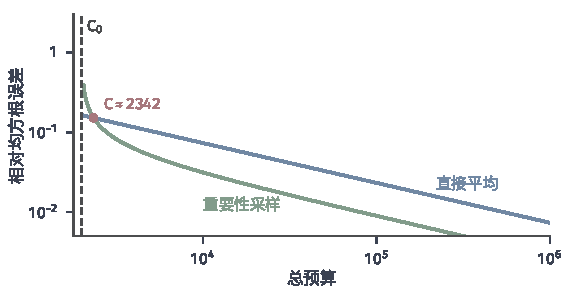
\includegraphics[width=96mm]{figures/07-probability/08-sampling-and-integration/matplotlib/vr-budget-crossover/figure.pdf}
 \caption{$I=\mathbb{P}(X>4)$，$X\sim\operatorname{Exp}(1)$，相对均方根误差$\sqrt{v\,c/(C-C_0)}/I$随总预算$C$的变化，双对数坐标。蓝线为直接平均（$v=0.01798$，$c=1$，$C_0=0$），绿线为第~\ref{sec:vr-change-distribution}节的加权估计（$v=0.001749$，$c=1.5$，$C_0=2000$），虚线标出$C_0$，红点为两者相等的预算。}
 \label{fig:vr-budget-crossover}
\end{BookInlineFigure}

\paragraph{二阶矩要逐项核对}
式~\eqref{eq:vr-work-variance}要求$v<\infty$。本章的每一种改动都会改变单元的形式：乘以权重、减去辅助量、换成条件平均或成对平均。原积分存在只说明$\mathbb{E}[\lvert Y\rvert]<\infty$，不说明$\mathbb{E}[Y^2]<\infty$。方差为无穷时，式~\eqref{eq:vr-relative-efficiency}失去意义，误差也不再按$m^{-1/2}$缩小。所以每引入一种估计量，都要单独检查它的二阶矩。

\paragraph{有偏的估计}
有些估计量不是无偏的，例如用同一批样本估计系数再代回，或者用两个平均值的比值作估计。这时比较的对象是均方误差，由第~\ref{chap:monte-carlo-integration-error}章，
\[
 \mathbb{E}\bigl[(\hat{I}-I)^2\bigr]=\bigl(\mathbb{E}[\hat{I}]-I\bigr)^2+\operatorname{Var}(\hat{I}) .
\]
常见的情形是偏差与$1/n$同阶而方差与$1/n$同阶，偏差的平方是$1/n^2$阶，样本量大时可以忽略。但样本量小时两者可能相当。另一个陷阱是：把内部样本量固定的有偏估计独立重复$R$次再平均，方差按$1/R$缩小，偏差却原样保留。这类估计的偏差要按内部样本量单独分析。

\paragraph{三个改动的位置}
一次随机计算可以看成一条流水线：基础随机数$\bm{U}$经生成映射$T$变成样本$X=T(\bm{U})$，求值得到$f(X)$，再取平均。图~\ref{fig:vr-three-routes}标出本章三类方法改动的位置。改变分布作用在生成这一步，样本改从别的分布抽取；改变计算公式作用在求值这一步，被平均的量不再是$f(X)$；改变抽样机制作用在基础随机数上，改变的是各个$\bm{U}$之间的安排。三类改动可以组合，组合后要按本节的口径重新检查期望、二阶矩和成本；在实际预算下怎样分配试运行与正式计算、怎样在方法之间取舍，由第~\ref{chap:sampling-budget-method-selection}章统一讨论。

\begin{BookInlineFigure}
 \centering
 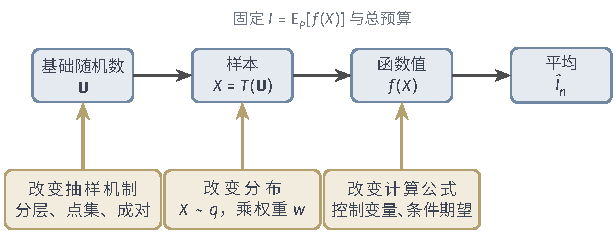
\includegraphics[width=104mm]{figures/07-probability/08-sampling-and-integration/tikz/vr-three-routes/figure.pdf}
 \caption{一次随机计算的流水线与三类方差控制方法的作用位置。上排是基础随机数、样本、函数值与平均；下排黄色框分别改动基础随机数的安排、样本的分布与被平均的量。积分$I$与总预算在比较中保持不变。}
 \label{fig:vr-three-routes}
\end{BookInlineFigure}


\section{改变分布}
\label{sec:vr-change-distribution}

尾概率$\mathbb{P}(X>4)$难算，是因为按$P$抽样时样本几乎从不进入尾部。一个自然的想法是换一个更常落进尾部的分布来抽样。这样抽到的样本不再服从$P$，直接求平均会高估尾概率；但每个样本被“多抽”了多少是已知的，可以按比例把它的贡献折回去。

用质量的语言说：$P$把单位质量按密度$p$摊在样本空间上，新分布把同样的单位质量按密度$q$重新摊开。一个按$q$抽到的样本点$x$，代表它附近$q$那么多的质量；要让它替$P$说话，就要给它乘上$p(x)/q(x)$。$q$比$p$大的地方样本来得勤，每个样本分量轻；$q$比$p$小的地方样本来得少，每个样本分量重。这种做法称为\term{重要性采样}（importance sampling）。本节先验证折算的公式，再研究怎样选择新分布，最后处理目标密度只知道到一个常数倍的情形。

\subsection{换测度与权重}
\label{sec:vr-change-of-measure}

设样本空间$\mathcal{X}$上有参考测度$\mu$：$\mathcal{X}=\mathbb{R}^{d}$时取Lebesgue测度，$\mathcal{X}$可数时取计数测度。目标分布$P$关于$\mu$有密度$p$，另取一个容易抽样、密度$q$可以计算的分布$Q$，称为建议分布（第~\ref{chap:sample-generation}章的拒绝采样已经用过这个名称）。

\begin{definition}[重要性采样估计]
\label{def:vr-importance-sampling}
设$\{x:f(x)p(x)\neq0\}\subseteq\{x:q(x)>0\}$（允许相差一个$\mu$零测集）。称
\begin{equation}
 w(x)=\begin{cases}p(x)/q(x), & q(x)>0,\\ 0, & q(x)=0\end{cases}
 \label{eq:vr-importance-weight}
\end{equation}
为\term{重要性权重}（importance weight）。对独立且都服从$Q$的$X_1,\dots,X_n$，称
\begin{equation}
 \hat{I}_n^{\mathrm{IS}}=\frac1n\sum_{i=1}^{n}f(X_i)\,w(X_i)
 \label{eq:vr-is-estimator}
\end{equation}
为$I$的重要性采样估计。
\end{definition}

定义中的包含关系称为覆盖条件：凡是$fp$不为零、对积分有贡献的地方，建议分布都必须有正密度。$q=0$处的权重取值无关紧要，因为按$Q$抽样几乎不会落到那里。

\begin{theorem}[换测度恒等式]
\label{thm:vr-change-of-measure}
设覆盖条件成立且$\mathbb{E}_P[\lvert f(X)\rvert]<\infty$。则$f w$在$Q$下可积，
\begin{equation}
 \mathbb{E}_Q[f(X)w(X)]=\mathbb{E}_P[f(X)]=I ,
 \label{eq:vr-change-of-measure}
\end{equation}
所以$\hat{I}_n^{\mathrm{IS}}$无偏，并且当$n\to\infty$时$\hat{I}_n^{\mathrm{IS}}\xrightarrow{\mathrm{a.s.}}I$。若进一步有
\begin{equation}
 M(q)=\mathbb{E}_Q\bigl[f(X)^2w(X)^2\bigr]=\int_{\{q>0\}}\frac{f^2p^2}{q}\,\mathrm{d}\mu<\infty ,
 \label{eq:vr-is-second-moment}
\end{equation}
则
\begin{equation}
 \operatorname{Var}\bigl(\hat{I}_n^{\mathrm{IS}}\bigr)=\frac{M(q)-I^2}{n} .
 \label{eq:vr-is-variance}
\end{equation}
\end{theorem}

\begin{proof}
记$S=\{q>0\}$。在$S$上$w\,q=p$，所以
\[
 \mathbb{E}_Q\bigl[\lvert f w\rvert\bigr]=\int_S\lvert f\rvert\frac{p}{q}\,q\,\mathrm{d}\mu=\int_S\lvert f\rvert p\,\mathrm{d}\mu .
\]
由覆盖条件，$S$之外$\lvert f\rvert p$几乎处处为零，右边等于$\mathbb{E}_P[\lvert f\rvert]<\infty$。去掉绝对值重复同样的计算，得到式~\eqref{eq:vr-change-of-measure}。

于是$f(X_i)w(X_i)$是独立同分布、期望为$I$的可积变量。对它们的平均取期望得到无偏性；由第~\ref{chap:laws-of-large-numbers}章的强大数律得到几乎必然收敛。二阶矩有限时，单项方差为$M(q)-I^2$，独立平均的方差除以$n$。
\end{proof}

在$S$上，$w$正是$P$相对于$Q$的密度，式~\eqref{eq:vr-change-of-measure}就是\BookChapterRef{chap:measure-densities}{卷四第8章“测度的密度”}中换测度公式的一个特例。定理的两部分条件不同：无偏和一致只需要原积分绝对收敛；方差有限需要式~\eqref{eq:vr-is-second-moment}，这是加权变量在$Q$下的二阶矩，与$f$在$P$下的二阶矩不是一回事。

\paragraph{手算一遍}
用导言的尾概率演示。目标$p(x)=\mathrm{e}^{-x}$（$x>0$），$f=\mathbf{1}_{\{x>4\}}$。取建议分布$Q=\operatorname{Exp}(1/4)$，平均值为$4$，比目标常进尾部。它的密度和权重是
\[
 q(x)=\tfrac14\mathrm{e}^{-x/4},\qquad w(x)=\frac{\mathrm{e}^{-x}}{\tfrac14\mathrm{e}^{-x/4}}=4\mathrm{e}^{-3x/4} .
\]
下面用五个均匀随机数逐步演示：
\[
 u=0.37,\quad 0.81,\quad 0.06,\quad 0.52,\quad 0.23 .
\]
按第~\ref{chap:sample-generation}章的逆分位数方法，$x=-4\ln u$服从$\operatorname{Exp}(1/4)$，得到
\[
 x_1=3.977,\quad x_2=0.843,\quad x_3=11.254,\quad x_4=2.616,\quad x_5=5.879 .
\]
只有$x_3$和$x_5$超过$4$，它们的权重分别是
\[
 w(x_3)=4\mathrm{e}^{-8.440}=0.00086,\qquad w(x_5)=4\mathrm{e}^{-4.409}=0.04867 .
\]
其余三项$f=0$。于是
\[
 \hat{I}_5^{\mathrm{IS}}=\frac{0.00086+0.04867}{5}=0.00991 .
\]
真值是$0.01832$。五个样本的估计当然粗糙，但它不是零。用同样五个$u$按$x=-\ln u$生成$\operatorname{Exp}(1)$样本，得到的五个值都小于$3$，直接平均给出$0$。

\begin{BookInlineFigure}
 \centering
 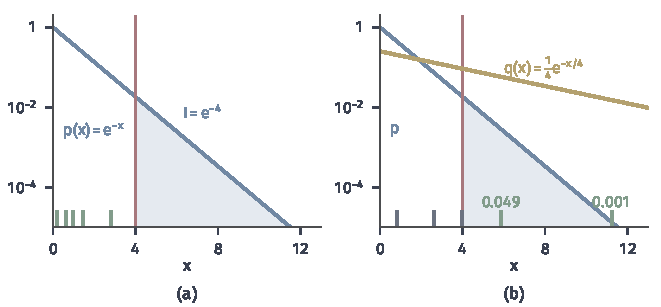
\includegraphics[width=112mm]{figures/07-probability/08-sampling-and-integration/matplotlib/vr-is-tail/figure.pdf}
 \caption{尾概率$I=\mathbb{P}(X>4)$的两种抽样，纵轴为对数刻度。蓝线为目标密度$p(x)=\mathrm{e}^{-x}$，浅蓝区域是$x>4$的尾部，红线是阈值。(a)用$u=0.37,0.81,0.06,0.52,0.23$按$x=-\ln u$生成的五个样本（绿色短线），全部落在阈值左侧。(b)同一组$u$按$x=-4\ln u$从黄线所示的$q$生成；越过阈值的两个样本为绿色并标出权重$w=4\mathrm{e}^{-3x/4}$，其余为灰色。}
 \label{fig:vr-is-tail}
\end{BookInlineFigure}

图~\ref{fig:vr-is-tail}对比了两种抽样。要算这一估计的方差，按式~\eqref{eq:vr-is-second-moment}在尾部积分：
\[
 M(q)=\int_4^{\infty}\frac{\mathrm{e}^{-2x}}{\tfrac14\mathrm{e}^{-x/4}}\,\mathrm{d}x=4\int_4^{\infty}\mathrm{e}^{-7x/4}\,\mathrm{d}x=\frac{16}{7}\mathrm{e}^{-7}\approx0.002084 .
\]
减去$I^2\approx0.000335$，单样本方差约为$0.001749$，只有直接平均的$0.01798$的$1/10.3$。这正是第~\ref{sec:vr-comparison}节例子中用到的数值。

\paragraph{覆盖条件去掉会怎样}
若建议分布只在$(0,6)$上有正密度，例如把$\operatorname{Exp}(1/4)$截断在$6$以内，$x>6$这部分尾部永远抽不到。重复定理的证明，估计的期望变为
\[
 \int_{\{q>0\}}f p\,\mathrm{d}\mu=\int_4^{6}\mathrm{e}^{-x}\,\mathrm{d}x=\mathrm{e}^{-4}-\mathrm{e}^{-6}\approx0.01584 ,
\]
比$I$少了$\mathrm{e}^{-6}/\mathrm{e}^{-4}\approx13.5\%$。这一偏差不随$n$减小，样本再多也只是越来越准地算出一个错误的数。

\paragraph{无偏而方差无穷}
仍对同一尾概率，改取$Q=\operatorname{Exp}(\lambda)$。对一般的$\lambda>0$，
\[
 M(q)=\int_4^{\infty}\frac{\mathrm{e}^{-2x}}{\lambda\mathrm{e}^{-\lambda x}}\,\mathrm{d}x=\frac1\lambda\int_4^{\infty}\mathrm{e}^{-(2-\lambda)x}\,\mathrm{d}x .
\]
$\lambda<2$时积分有限；$\lambda\geq2$时被积函数不衰减，$M(q)=\infty$。覆盖条件对每个$\lambda$都成立，所以估计都无偏、都收敛；但$\lambda\geq2$时方差为无穷。

$\lambda=2.5$时问题看得很清楚。建议样本进入尾部的概率只有$\mathrm{e}^{-10}\approx4.5\times10^{-5}$，而一旦进入，权重$w=0.4\mathrm{e}^{1.5x}$至少是$0.4\mathrm{e}^{6}\approx161$。估计值大部分时间是零，偶尔被一个巨大的权重拉高。图~\ref{fig:vr-is-running-mean}比较了两种$\lambda$下的运行平均：$\lambda=1/4$的三条路径平稳地收拢到真值；$\lambda=2.5$的三条路径在$n=2\times10^{5}$时分别只有$8$、$9$、$16$个尾部样本，终值为真值的$0.85$、$0.67$、$1.41$倍，路径呈台阶状跳动。

\begin{BookInlineFigure}
 \centering
 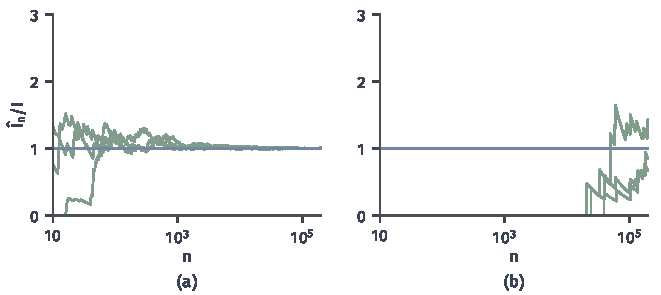
\includegraphics[width=112mm]{figures/07-probability/08-sampling-and-integration/matplotlib/vr-is-running-mean/figure.pdf}
 \caption{重要性采样估计的运行平均除以真值$I=\mathrm{e}^{-4}$，横轴为样本数（对数刻度），每图三条路径（种子11、12、13）。(a)$Q=\operatorname{Exp}(1/4)$，加权变量方差有限；(b)$Q=\operatorname{Exp}(2.5)$，估计仍无偏但加权变量的二阶矩为无穷。蓝线标出比值$1$。}
 \label{fig:vr-is-running-mean}
\end{BookInlineFigure}

\subsection{建议分布的选择}
\label{sec:vr-proposal-choice}

上一小节说明，权重公式正确只保证无偏；估计好不好，取决于式~\eqref{eq:vr-is-second-moment}的二阶矩$M(q)$。选择建议分布分两步。先从$M(q)$出发问：什么样的$q$最好？答案通常无法直接使用，于是再问：怎样用一次试运行拟合出一个可用的$q$，并且不破坏正式估计的性质？

\subsubsection{理想建议分布}
\label{sec:vr-ideal-proposal}

单样本方差是$M(q)-I^2$，其中$I$与$q$无关，所以比较建议分布就是比较$M(q)$。式~\eqref{eq:vr-is-second-moment}的被积函数是$f^2p^2/q$：分子大的地方，$q$也必须大，否则这一项会被放大。分子由$\lvert f\rvert p$决定，它衡量的是每个位置对积分的贡献，而不是样本在$P$下出现的频繁程度。

\begin{theorem}[理想建议分布]
\label{thm:vr-ideal-proposal}
设$0<\mathbb{E}_P[\lvert f(X)\rvert]<\infty$。对每个满足覆盖条件的密度$q$，
\begin{equation}
 M(q)\geq\bigl(\mathbb{E}_P[\lvert f(X)\rvert]\bigr)^2 ,
 \label{eq:vr-is-lower-bound}
\end{equation}
等号当且仅当$q$与
\begin{equation}
 q^{*}(x)=\frac{\lvert f(x)\rvert\,p(x)}{\mathbb{E}_P[\lvert f(X)\rvert]}
 \label{eq:vr-ideal-proposal}
\end{equation}
$\mu$几乎处处相等时成立。
\end{theorem}

\begin{proof}
记$S=\{q>0\}$，$a=\mathbb{E}_P[\lvert f\rvert]$。由覆盖条件，$a=\int_S\lvert f\rvert p\,\mathrm{d}\mu$。把被积函数拆成两个因子，用Cauchy--Schwarz不等式：
\[
 a=\int_S\frac{\lvert f\rvert p}{\sqrt{q}}\cdot\sqrt{q}\,\mathrm{d}\mu\leq\Bigl(\int_S\frac{f^2p^2}{q}\,\mathrm{d}\mu\Bigr)^{1/2}\Bigl(\int_S q\,\mathrm{d}\mu\Bigr)^{1/2} .
\]
右边第二个因子是$1$，第一个因子是$M(q)^{1/2}$，平方即得式~\eqref{eq:vr-is-lower-bound}。

等号成立当且仅当两个因子在$S$上几乎处处成比例，即存在常数$k$使$\lvert f\rvert p=k\,q$在$S$上几乎处处成立。两边在$S$上积分，得$k=a$，所以$q=\lvert f\rvert p/a$在$S$上几乎处处成立。在$S$之外$q=0$，而由覆盖条件$\lvert f\rvert p$也几乎处处为零。所以$q=q^{*}$几乎处处成立。反过来，$q=q^{*}$时直接计算得$M(q^{*})=a^2$。
\end{proof}

最小的单样本方差是$a^2-I^2$。$f$在$P$下几乎必然不变号时$\lvert I\rvert=a$，最小方差为零：每个样本的$f w$恰好等于$I$。$f$变号时$a>\lvert I\rvert$，即使用理想建议，方差也不为零。

\paragraph{尾概率：零方差与循环}
尾概率中$f=\mathbf{1}_{\{x>4\}}$不变号，$a=I=\mathrm{e}^{-4}$，理想建议是
\[
 q^{*}(x)=\frac{\mathrm{e}^{-x}\mathbf{1}_{\{x>4\}}}{\mathrm{e}^{-4}}=\mathrm{e}^{-(x-4)}\mathbf{1}_{\{x>4\}} ,
\]
也就是在$X>4$条件下$X$的分布。按它抽样，每个样本都落在尾部，权重是常数：
\[
 w(x)=\frac{\mathrm{e}^{-x}}{\mathrm{e}^{-(x-4)}}=\mathrm{e}^{-4},\qquad x>4 .
\]
一个样本就给出精确的$I$。问题在于$q^{*}$的归一化常数正是$a=I$：写出$q^{*}$，等于已经知道了答案。这里能写出来，只是因为指数分布的尾部恰好还是指数分布。一般地，理想建议告诉我们抽样应当往哪里集中，而不是一个可以直接使用的分布。

\paragraph{变号的被积函数}
取$P=\mathcal{N}(0,1)$，$f(x)=x$，$I=0$。此时$a=\mathbb{E}\lvert X\rvert=\sqrt{2/\pi}$，理想建议
\[
 q^{*}(x)=\frac{\lvert x\rvert\varphi(x)}{\sqrt{2/\pi}}
\]
在原点处为零、在$\pm1$附近各有一个峰。它的单样本方差是
\[
 a^2-I^2=\frac{2}{\pi}\approx0.637 ,
\]
比直接平均的$\operatorname{Var}(X)=1$小，但不为零：正负两部分的样本各自带着符号，平均时仍有波动。若把$f$拆成正部$f^{+}=\max\{f,0\}$与负部$f^{-}=\max\{-f,0\}$，分别用各自的理想建议计算再相减，两部分都是零方差。图~\ref{fig:vr-ideal-proposal}画出两个例子中的$p$、贡献$\lvert f\rvert p$与$q^{*}$。

\begin{BookInlineFigure}
 \centering
 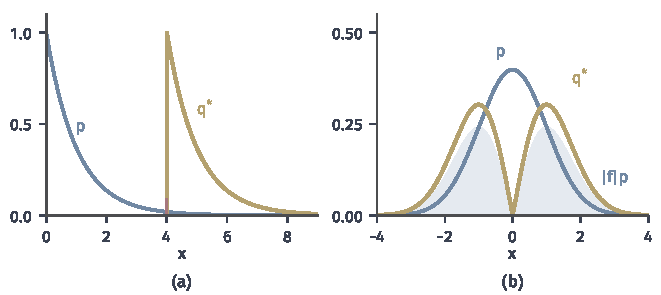
\includegraphics[width=112mm]{figures/07-probability/08-sampling-and-integration/matplotlib/vr-ideal-proposal/figure.pdf}
 \caption{理想建议分布$q^{*}=\lvert f\rvert p/\mathbb{E}_P\lvert f\rvert$（黄线）与目标密度$p$（蓝线）。(a)$p(x)=\mathrm{e}^{-x}$，$f=\mathbf{1}_{\{x>4\}}$：$q^{*}$是平移到$4$的指数密度，贡献$\lvert f\rvert p$为$x>4$下方面积$\mathrm{e}^{-4}$，在此刻度下几乎看不见。(b)$p=\mathcal{N}(0,1)$，$f(x)=x$：浅蓝区域为$\lvert x\rvert\varphi(x)$，$q^{*}$是它除以$\sqrt{2/\pi}$，在原点为零。}
 \label{fig:vr-ideal-proposal}
\end{BookInlineFigure}

\paragraph{在分布族内选择}
既然$q^{*}$通常不可用，退一步在一个可采样的族中找使$M(q)$最小的成员。尾概率中取$Q=\operatorname{Exp}(\lambda)$，上一小节已经算出，$0<\lambda<2$时
\begin{equation}
 v(\lambda)=M(q_\lambda)-I^2=\frac{\mathrm{e}^{-4(2-\lambda)}}{\lambda(2-\lambda)}-\mathrm{e}^{-8} .
 \label{eq:vr-exp-family-variance}
\end{equation}
对第一项取对数，得到$4\lambda-8-\ln\lambda-\ln(2-\lambda)$，令它的导数为零：
\[
 4-\frac1\lambda+\frac{1}{2-\lambda}=0 .
\]
两边乘$\lambda(2-\lambda)$整理，得
\[
 4\lambda^2-10\lambda+2=0 .
\]
在$(0,2)$内的根是$\lambda^{*}=(5-\sqrt{17})/4\approx0.219$，此时$v(\lambda^{*})\approx0.001730$，比直接平均小$10.4$倍。$\lambda^{*}$对应的平均值$1/\lambda^{*}\approx4.56$略大于阈值$4$：抽样集中在尾部的起点附近，那里正是$\lvert f\rvert p$最大的地方。

\begin{BookInlineFigure}
 \centering
 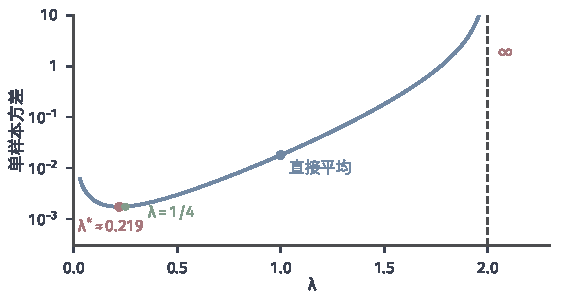
\includegraphics[width=96mm]{figures/07-probability/08-sampling-and-integration/matplotlib/vr-is-second-moment/figure.pdf}
 \caption{尾概率$\mathbb{P}(X>4)$用$Q=\operatorname{Exp}(\lambda)$作建议时的单样本方差$v(\lambda)$，纵轴为对数刻度。蓝点$\lambda=1$即直接平均，红点为最优$\lambda^{*}\approx0.219$，绿点为正文例子用的$\lambda=1/4$；虚线$\lambda=2$右侧方差为无穷。}
 \label{fig:vr-is-second-moment}
\end{BookInlineFigure}

图~\ref{fig:vr-is-second-moment}画出$v(\lambda)$。曲线有两个陡峭的方向。$\lambda\to0$时建议分布摊得过宽，大部分样本落在远离阈值、贡献极小的地方；$\lambda\to2$时建议分布的尾部衰减得和$p^2$一样快，权重平方在远处不再衰减，二阶矩发散。后一种情形是更危险的一侧：它不表现为估计变差一点，而是方差直接变为无穷。

\paragraph{尾部过轻}
这个现象有一般的形式。$f$有界时，$M(q)\leq\sup\lvert f\rvert^2\,\mathbb{E}_P[w]$，若$q$的尾部至少和$p$一样重，使$w=p/q$有界，则$M(q)$有限。反之，若在某个方向上$q$比$p$衰减得快很多，$w$在那里无界，$f^2p^2/q$可能不可积。所以选建议分布时，宁可尾部偏重，不可偏轻。

\subsubsection{试运行中的拟合}
\label{sec:vr-pilot-fitting}

当理想建议无法直接写出时，可以先用一个覆盖面足够宽的分布$q_0$做一次试运行，从试运行样本中看出贡献集中在哪里，再从一个可采样、密度可计算的族中挑出与$q^{*}$相近的成员。

\paragraph{主要思想}
设$Y_1,\dots,Y_m$独立且都服从$q_0$，$q_0$覆盖$fp$。记
\begin{equation}
 c_j=\frac{\lvert f(Y_j)\rvert\,p(Y_j)}{q_0(Y_j)},\qquad j=1,\dots,m .
 \label{eq:vr-pilot-contribution}
\end{equation}
由换测度恒等式，对任意使积分存在的函数$g$，
\[
 \mathbb{E}_{q_0}\bigl[c\,g(Y)\bigr]=\int\lvert f\rvert p\,g\,\mathrm{d}\mu=a\,\mathbb{E}_{q^{*}}[g] .
\]
所以以$c_j$为权重的加权平均$\sum_j c_jg(Y_j)/\sum_j c_j$近似$\mathbb{E}_{q^{*}}[g]$：带权重$c_j$的试运行样本是$q^{*}$的一个粗略画像，$c_j$可以看成第$j$个试运行点对积分的贡献。

拟合时在族中挑出各项矩与这个画像一致的成员。以方差为$1$的正态位置族$\mathcal{N}(m,1)$为例，与$q^{*}$的KL散度为
\[
 D_{\mathrm{KL}}\bigl(q^{*}\Vert\mathcal{N}(m,1)\bigr)=\int q^{*}\ln q^{*}\,\mathrm{d}x+\frac12\ln(2\pi)+\frac12\mathbb{E}_{q^{*}}\bigl[(X-m)^2\bigr] .
\]
只有最后一项依赖$m$，它在$m=\mathbb{E}_{q^{*}}[X]$时最小。把$\mathbb{E}_{q^{*}}[X]$换成加权平均，就得到以贡献为权重的均值。用KL散度逼近一个分布的一般讨论见第~\ref{chap:distribution-approximation}章。

贡献集中在几个分离的区域时，每个区域配一个成分，成分的权重取该区域贡献所占的比例。再留一份$q_0$本身作为\term{防御性混合}（defensive mixture）成分：
\begin{equation}
 q=\alpha\,q_0+(1-\alpha)\sum_{k=1}^{K}\pi_k\,\mathcal{N}(m_k,1),\qquad 0<\alpha<1 .
 \label{eq:vr-defensive-mixture}
\end{equation}
这一份保证了$q\geq\alpha q_0$，于是$w=p/q\leq p/(\alpha q_0)$：只要$p/q_0$有界，权重就有界，拟合得再差，二阶矩也不会发散；试运行没有看到的区域，也仍以$\alpha q_0$的密度被抽到。

\paragraph{计算过程}
下面结合一个两区域的例子写出计算过程。目标$P=\mathcal{N}(0,1)$，
\[
 f(x)=\mathbf{1}_{\{x<-2.5\}}+\mathbf{1}_{\{x>3\}} ,
\]
真值$I=\Phi(-2.5)+1-\Phi(3)=0.006210+0.001350=0.007560$，左侧贡献占$82\%$。直接平均的单样本方差为$I(1-I)\approx0.007502$。

\needspace{6\baselineskip}
\paragraph{变量}
\begin{itemize}
 \item 试运行分布$q_0$与试运行样本$Y_1,\dots,Y_m$；例中$q_0=\mathcal{N}(0,3^2)$，$m=30$。
 \item 贡献$c_j$，按式~\eqref{eq:vr-pilot-contribution}计算，长度为$m$的非负数组。
 \item 区域划分及区域数$K$；例中按符号分为左右两区，$K=2$。
 \item 拟合参数：成分权重$\pi_k$与成分均值$m_k$，$k=1,\dots,K$；防御比例$\alpha$，例中$\alpha=0.2$。
\end{itemize}

\needspace{6\baselineskip}
\paragraph{步骤}
\begin{enumerate}
 \item \textbf{试运行。}抽取$Y_1,\dots,Y_m\sim q_0$，计算各$c_j$。例中（种子3）$30$个点里有$9$个落进贡献区，其中只有$4$个的贡献不可忽略：
 \[
 \begin{array}{lcccc}
  y_j & -3.165 & -2.596 & 3.007 & 4.637\\
  c_j & 0.03492 & 0.15020 & 0.05394 & 0.00021
 \end{array}
 \]
 另外$5$个点落在$\lvert y\rvert>5.8$处，那里$p$极小，贡献都小于$10^{-6}$。

 \item \textbf{按区域汇总。}对每个区域$k$计算贡献之和$s_k$。例中
 \[
  s_1=0.03492+0.15020=0.18512,\qquad s_2=0.05394+0.00021=0.05415 .
 \]

 \item \textbf{成分权重。}取$\pi_k=s_k/\sum_l s_l$。例中
 \[
  \pi_1=\frac{0.18512}{0.23927}=0.774,\qquad \pi_2=0.226 .
 \]
 真实比例是$0.821$与$0.179$，三十个试运行点给出的估计已经大致正确。

 \item \textbf{成分均值。}取$m_k=\sum_{j\in k}c_jy_j/s_k$。例中
 \[
  m_1=\frac{0.03492\times(-3.165)+0.15020\times(-2.596)}{0.18512}=-2.703 ,
 \]
 同样算得$m_2=3.013$。

 \item \textbf{组装建议。}代入式~\eqref{eq:vr-defensive-mixture}。例中
 \[
  q=0.2\,\mathcal{N}(0,3^2)+0.8\bigl[0.774\,\mathcal{N}(-2.703,1)+0.226\,\mathcal{N}(3.013,1)\bigr] .
 \]
\end{enumerate}
最终得到的$q$由数值积分算得单样本方差$M(q)-I^2\approx1.99\times10^{-4}$，是直接平均的$1/37.7$。这里$p/q_0=3\mathrm{e}^{-4x^2/9}\leq3$，所以权重不超过$3/\alpha=15$。图~\ref{fig:vr-mixture-fit}左图是试运行点及其贡献，右图把拟合的$q$与$q^{*}$放在一起。

\begin{BookInlineFigure}
 \centering
 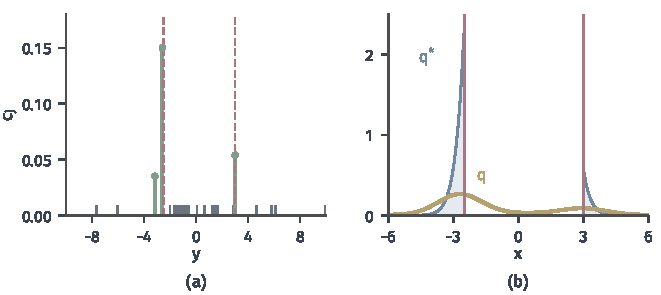
\includegraphics[width=112mm]{figures/07-probability/08-sampling-and-integration/matplotlib/vr-mixture-fit/figure.pdf}
 \caption{两区域贡献的建议拟合，$P=\mathcal{N}(0,1)$，$f=\mathbf{1}_{\{x<-2.5\}}+\mathbf{1}_{\{x>3\}}$，红色虚线或实线为两个阈值。(a)$q_0=\mathcal{N}(0,3^2)$的$30$个试运行点（种子3）：灰色短线为贡献可忽略的点，绿色竖线高度为贡献$c_j$。(b)蓝线与浅蓝区域为理想建议$q^{*}=fp/I$，黄线为拟合的防御性混合$q$。}
 \label{fig:vr-mixture-fit}
\end{BookInlineFigure}

\paragraph{没看到不等于没有}
试运行的范围不够时，拟合会漏掉区域。把试运行分布换成较窄的$q_0=\mathcal{N}(0,1.5^2)$，同样抽$30$个点（种子0），只有一个点$-3.488$落进左区，没有点越过$3$。按上面的步骤只能拟合出左侧一个成分$\mathcal{N}(-3.488,1)$。若不留防御成分，右区$x>3$只能靠这个远在左边的成分偶尔覆盖，单样本方差约为$1.3\times10^{5}$，是直接平均的$1.8\times10^{7}$倍；留下$\alpha=0.2$的$q_0$后，方差降为约$7.4\times10^{-4}$，仍比直接平均好约$10$倍。试运行中某个区域一个点也没有，只说明$m$个点没有落到那里，不说明那里对积分没有贡献。

\subsubsection{固定建议后的估计}
\label{sec:vr-fixed-proposal}

拟合出的$q$依赖试运行样本，本身是随机的。正式估计必须说明：在$q$随机的情况下，加权平均还是否无偏、方差怎样计算。

把试运行的全部结果记为$D=(Y_1,\dots,Y_m)$，拟合的建议记为$q_D$。正式计算在给定$D$后，用一组与$D$独立的新随机数抽取$X_1,\dots,X_n\sim q_D$，再计算
\[
 \hat{I}_n^{\mathrm{IS}}=\frac1n\sum_{i=1}^{n}f(X_i)\frac{p(X_i)}{q_D(X_i)} .
\]
图~\ref{fig:vr-two-stage}画出这一两阶段结构。

\begin{BookInlineFigure}
 \centering
 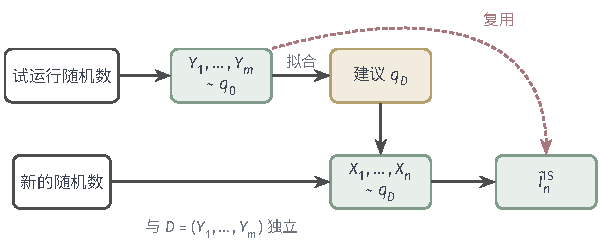
\includegraphics[width=102mm]{figures/07-probability/08-sampling-and-integration/tikz/vr-two-stage/figure.pdf}
 \caption{两阶段重要性采样。试运行随机数产生$D=(Y_1,\dots,Y_m)$并拟合建议$q_D$；正式样本由与$D$独立的新随机数按$q_D$生成。红色虚线表示把试运行点直接混入正式估计，这样做会破坏下面的条件无偏性。}
 \label{fig:vr-two-stage}
\end{BookInlineFigure}

\begin{theorem}[两阶段估计的无偏性]
\label{thm:vr-two-stage}
设$\mathbb{E}_P[\lvert f\rvert]<\infty$，对几乎每个试运行结果$D$，$q_D$都覆盖$fp$，且正式样本所用的随机数与$D$独立。则
\begin{equation}
 \mathbb{E}\bigl[\hat{I}_n^{\mathrm{IS}}\bigm|D\bigr]=I,\qquad \mathbb{E}\bigl[\hat{I}_n^{\mathrm{IS}}\bigr]=I .
 \label{eq:vr-two-stage-unbiased}
\end{equation}
若再有$\mathbb{E}[M(q_D)]<\infty$，则
\begin{equation}
 \operatorname{Var}\bigl(\hat{I}_n^{\mathrm{IS}}\bigr)=\frac{\mathbb{E}[M(q_D)]-I^2}{n} .
 \label{eq:vr-two-stage-variance}
\end{equation}
\end{theorem}

\begin{proof}
正式样本可以写成$X_i=T(D,\bm{U}_i)$，其中$\bm{U}_1,\dots,\bm{U}_n$与$D$独立，且对固定的$d$，$T(d,\bm{U}_i)$服从$q_d$。由第~\ref{chap:conditional-distributions}章，$\bm{U}_i$与$D$独立时，给定$D=d$的条件期望可以把$d$代入后只对$\bm{U}_i$求期望。对固定的$d$，这是建议$q_d$下的普通重要性采样，由定理~\ref{thm:vr-change-of-measure}，它的期望是$I$。这就是式~\eqref{eq:vr-two-stage-unbiased}的第一式；再用全期望公式得到第二式。

同样，给定$D=d$时的条件方差是$(M(q_d)-I^2)/n$。由全方差公式，总方差等于条件方差的期望加条件期望的方差；条件期望恒为$I$，后一项为零，于是得到式~\eqref{eq:vr-two-stage-variance}。
\end{proof}

定理中两个条件的作用不同。“对每个$D$都覆盖”保证无论试运行结果如何，正式估计都不偏；防御性混合使这一条自动成立，因为$q_D\geq\alpha q_0$而$q_0$覆盖$fp$。“新随机数与$D$独立”保证条件化以后正式样本确实服从$q_D$。在固定$D$下，正式样本的$f w$值独立同分布，用它们的样本方差除以$n$就可以估计条件方差。

\paragraph{复用试运行点}
如果把试运行点$Y_j$也代入同一个加权公式，即在正式平均中加入$f(Y_j)p(Y_j)/q_D(Y_j)$，问题出在两处：$Y_j$并不服从$q_D$，而是服从$q_0$；$q_D$又是由$Y_j$拟合出来的，在$Y_j$附近往往偏大。这一项的期望一般不等于$I$。试运行点可以利用，但要用它实际来源的密度：$f$非负时，$\sum_jc_j/m$就是基于$q_0$的一个无偏估计，例中为$0.00798$。正式估计在给定$D$时的条件期望恒为$I$，所以两者不相关，可以按固定的比例合并。

\paragraph{混合形式不保证有限方差}
式~\eqref{eq:vr-two-stage-variance}要求$\mathbb{E}[M(q_D)]<\infty$，这要对试运行的每种可能结果检查。混合本身不能保证这一点。仍用上面的两区域例子，如果在步骤4中同时用加权方差拟合每个成分的方差，左右两个成分的标准差分别只有$0.223$与$0.103$。没有防御成分时，$q$在远处按$\mathrm{e}^{-x^2/(2\times0.223^2)}$衰减，比$p^2\propto\mathrm{e}^{-x^2}$快得多，左区上$p^2/q$不可积，$M(q)=\infty$。加上$\alpha=0.2$的$q_0=\mathcal{N}(0,3^2)$后，权重有界，单样本方差约为$7.7\times10^{-5}$。起作用的是一个尾部足够重的成分，而不是混合这一形式。

试运行越长，拟合越可靠，但它的成本也计入总预算。试运行与正式计算之间怎样分配预算，由第~\ref{chap:sampling-budget-method-selection}章讨论。

\subsection{自归一化估计}
\label{sec:vr-self-normalized}

许多目标分布只知道到一个常数倍：能算$\widetilde{p}(x)\geq0$，而$p=\widetilde{p}/Z$中的归一化常数
\[
 Z=\int\widetilde{p}\,\mathrm{d}\mu,\qquad 0<Z<\infty
\]
无法直接计算。第~\ref{chap:sample-generation}章的拒绝采样与Metropolis--Hastings采样都只用到$\widetilde{p}$。这时权重$p/q$算不出来，只能算$\widetilde{w}=\widetilde{p}/q=Zw$。

办法是用同一批样本同时估计$Z$。由换测度恒等式，$\mathbb{E}_Q[\widetilde{w}]=Z$，$\mathbb{E}_Q[\widetilde{w}f]=ZI$，两者相除，未知的$Z$约去。

\begin{definition}[自归一化估计]
\label{def:vr-self-normalized}
设$q$覆盖整个目标，即$\{\widetilde{p}>0\}\subseteq\{q>0\}$。对独立且都服从$Q$的$X_1,\dots,X_n$，记$\widetilde{w}_i=\widetilde{p}(X_i)/q(X_i)$，称
\begin{equation}
 \hat{I}_n^{\mathrm{SN}}=\frac{\sum_{i=1}^{n}\widetilde{w}_i\,f(X_i)}{\sum_{i=1}^{n}\widetilde{w}_i}
 \label{eq:vr-self-normalized}
\end{equation}
为\term{自归一化重要性采样}（self-normalized importance sampling）估计；分母为零时规定估计值为$0$。
\end{definition}

覆盖的要求比定义~\ref{def:vr-importance-sampling}更强：分母要估计整个$Z$，所以凡是$\widetilde{p}>0$的地方都要覆盖，不能只覆盖$f\widetilde{p}\neq0$的部分。

\begin{theorem}[自归一化估计的一致性]
\label{thm:vr-sn-consistency}
设$q$覆盖整个目标且$\mathbb{E}_P[\lvert f\rvert]<\infty$。则$\hat{I}_n^{\mathrm{SN}}\xrightarrow{\mathrm{a.s.}}I$。
\end{theorem}

\begin{proof}
由换测度恒等式，$\widetilde{w}$与$\widetilde{w}f$在$Q$下可积，期望分别是$Z$与$ZI$。由强大数律，几乎必然有
\[
 \frac1n\sum_{i=1}^{n}\widetilde{w}_i\to Z,\qquad \frac1n\sum_{i=1}^{n}\widetilde{w}_if(X_i)\to ZI .
\]
因为$Z>0$，在这些样本点上分母从某个$n$起为正，比值收敛到$ZI/Z=I$。
\end{proof}

\paragraph{有限样本的偏差}
比值的期望一般不是期望的比值。最极端的情形是$n=1$：只要$\widetilde{w}_1>0$，式~\eqref{eq:vr-self-normalized}就等于$f(X_1)$，于是估计的期望是$f$在$Q$下（限制在$\widetilde{w}>0$上）的平均，而不是在$P$下的平均。另一种有限样本现象是分母为零：若$\widetilde{p}$在$q$的支撑上有一部分为零，所有样本都可能落在那里，这时估计没有信息。

用一个能手算的例子看这些量。目标$\widetilde{p}(x)=x^2\mathrm{e}^{-x}$（$x>0$），它是$\operatorname{Gamma}(3,1)$的未归一化密度，$Z=2$；要算$I=\mathbb{E}_P[X]=3$。建议$Q=\operatorname{Exp}(1/2)$，于是
\[
 q(x)=\tfrac12\mathrm{e}^{-x/2},\qquad \widetilde{w}(x)=2x^2\mathrm{e}^{-x/2} .
\]
$n=1$时估计的期望是$\mathbb{E}_Q[X]=2$，偏差为$-1$。仍用前面那五个均匀数，按$x=-2\ln u$生成五个建议样本：
\[
 x=1.989,\quad 0.421,\quad 5.627,\quad 1.308,\quad 2.939 .
\]
对应的权重为
\[
 \widetilde{w}=2.926,\quad 0.288,\quad 3.799,\quad 1.779,\quad 3.974 .
\]
权重和为$12.766$，加权和$\sum\widetilde{w}_ix_i=41.326$，于是
\[
 \hat{I}_5^{\mathrm{SN}}=\frac{41.326}{12.766}=3.237 .
\]
副产品是$Z$的无偏估计$12.766/5=2.553$。

\paragraph{渐近误差}
把误差写成
\[
 \hat{I}_n^{\mathrm{SN}}-I=\frac{\frac1n\sum_{i=1}^{n}\widetilde{w}_i\bigl(f(X_i)-I\bigr)}{\frac1n\sum_{i=1}^{n}\widetilde{w}_i} .
\]
分子是独立同分布变量$\widetilde{w}(f-I)$的平均，它的期望是$ZI-IZ=0$。若中心化加权量的二阶矩
\begin{equation}
 \tau^2=\mathbb{E}_Q\bigl[\widetilde{w}(X)^2\bigl(f(X)-I\bigr)^2\bigr]<\infty ,
 \label{eq:vr-sn-tau}
\end{equation}

由第~\ref{chap:central-limit-theorem}章的中心极限定理，分子乘以$\sqrt{n}$依分布收敛到$\mathcal{N}(0,\tau^2)$；分母几乎必然收敛到$Z$。由第~\ref{chap:weak-convergence-of-distributions}章的Slutsky定理，
\begin{equation}
 \sqrt{n}\,\bigl(\hat{I}_n^{\mathrm{SN}}-I\bigr)\xrightarrow{\mathrm{d}}\mathcal{N}\Bigl(0,\frac{\tau^2}{Z^2}\Bigr) .
 \label{eq:vr-sn-clt}
\end{equation}
要检查的是$\widetilde{w}(f-I)$的二阶矩，而不是$\widetilde{w}f$的二阶矩：减去$I$以后，大权重落在$f\approx I$处的样本不再放大误差。式~\eqref{eq:vr-sn-clt}是渐近结论，它不给出任何固定$n$下的覆盖保证。

把分母写成$Z(1+\delta)$，$\delta$是分母的相对误差，展开$1/(1+\delta)\approx1-\delta$并取期望，可以得到偏差的主项：
\begin{equation}
 \mathbb{E}\bigl[\hat{I}_n^{\mathrm{SN}}\bigr]-I\approx-\frac{\mathbb{E}_Q\bigl[\widetilde{w}^2(f-I)\bigr]}{nZ^2} .
 \label{eq:vr-sn-bias}
\end{equation}
它是分子与分母协方差的结果。这只是主项：严格化需要控制分母接近零的事件以及展开的余项。例中数值积分给出$\tau^2/Z^2\approx3.687$，偏差系数$\approx-0.527$。偏差的平方与$1/n^2$同阶，方差与$1/n$同阶，样本量大时偏差可以忽略。图~\ref{fig:vr-snis}(a)用$4\times10^{4}$次独立重复验证了这两个阶：$n\geq8$时偏差与$0.527/n$吻合，$n=2$时偏差约为$0.48$，主项公式在这样小的样本下并不准确。顺便比较，直接从$\operatorname{Gamma}(3,1)$抽样时单样本方差是$3$，这里的渐近方差$3.687$稍大。

\begin{BookInlineFigure}
 \centering
 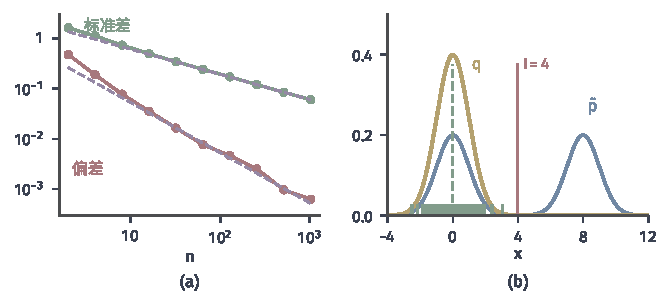
\includegraphics[width=112mm]{figures/07-probability/08-sampling-and-integration/matplotlib/vr-snis/figure.pdf}
 \caption{自归一化估计的偏差与覆盖问题。(a)目标$\operatorname{Gamma}(3,1)$，$f(x)=x$，建议$\operatorname{Exp}(1/2)$；每个$n$独立重复$4\times10^{4}$次（种子5），绿线为估计的标准差，红线为偏差的绝对值，紫色虚线为渐近参照$\sqrt{3.687/n}$与$0.527/n$。(b)目标$\widetilde{p}=\tfrac12\varphi(x)+\tfrac12\varphi(x-8)$（蓝线），建议$\mathcal{N}(0,1)$（黄线）；绿色短线为前$200$个建议样本，绿色虚线为$n=1000$时的估计值，红线为真值$4$。}
 \label{fig:vr-snis}
\end{BookInlineFigure}

\paragraph{权重的有效样本量看不到漏掉的区域}
实践中常用权重计算
\[
 n_{\mathrm{w}}=\frac{\bigl(\sum_{i=1}^{n}\widetilde{w}_i\bigr)^2}{\sum_{i=1}^{n}\widetilde{w}_i^2} .
\]
它介于$1$与$n$之间：权重全相等时为$n$，一个权重压倒其余时接近$1$。上面的五点例子中$n_{\mathrm{w}}=3.88$。它衡量的是已经抽到的样本之间权重的分散程度，看不到没有抽到的地方。

图~\ref{fig:vr-snis}(b)是一个反例。目标是两个相距$8$的正态峰的等权混合，真值$\mathbb{E}_P[X]=4$；建议$\mathcal{N}(0,1)$只盖住左峰。覆盖条件成立（$q$处处为正），所以定理~\ref{thm:vr-sn-consistency}保证估计最终收敛到$4$。但权重
\[
 \widetilde{w}(x)=\tfrac12+\tfrac12\mathrm{e}^{8x-32}
\]
只在$x>4$附近才明显偏离$\tfrac12$，而建议样本进入那里的概率约为$3\times10^{-5}$。$n=1000$（种子6）时，估计值为$-0.012$，而$n_{\mathrm{w}}=1000.0$：所有权重几乎相同，指标显示“完美”，估计却错了整整一个峰。经验指标稳定不能证明建议分布覆盖了目标的重要区域。


\section{改变计算公式}
\label{sec:vr-change-formula}

上一节保持被平均的对象不变，改变样本从哪里来。本节反过来：样本仍按$P$抽取，但不再直接平均$f(X)$，而是平均另一个期望同为$I$、波动更小的量。构造这样的量有两条路。一是找一个与$f$同步起伏、期望已知的辅助量，把可以预测的那部分波动减掉；二是把输入中的一部分随机性用条件平均精确地算掉，只对剩下的部分抽样。两种做法都会增加每个样本的计算，比较时要按第~\ref{sec:vr-comparison}节计入成本。

\subsection{控制变量}
\label{sec:vr-control-variates}

回到导言的第二个例子：
\[
 I=\int_0^1\mathrm{e}^{u}\,\mathrm{d}u=\mathrm{e}-1 .
\]
按$U\sim\operatorname{Unif}(0,1)$抽样，$\mathrm{e}^{U}$的方差为
\[
 \sigma^2=\mathbb{E}\bigl[\mathrm{e}^{2U}\bigr]-(\mathrm{e}-1)^2=\frac{\mathrm{e}^2-1}{2}-(\mathrm{e}-1)^2\approx0.2420 .
\]
这些波动的主要来源一目了然：$U$偏大，$\mathrm{e}^{U}$就偏大。而$U$本身的期望$1/2$是已知的。如果某次抽到的$U$比$1/2$大了$0.1$，就可以预先判断$\mathrm{e}^{U}$大约偏高了$0.1$乘以某个斜率，把这一部分减掉。

\begin{definition}[控制变量估计]
\label{def:vr-control-variate}
设$h$是一个在$P$下期望$\mu_h=\mathbb{E}_P[h(X)]$已知的函数，$\beta$为实数。对独立且都服从$P$的$X_1,\dots,X_n$，称
\begin{equation}
 \hat{I}_n^{\mathrm{CV}}(\beta)=\frac1n\sum_{i=1}^{n}\Bigl[f(X_i)-\beta\bigl(h(X_i)-\mu_h\bigr)\Bigr]
 \label{eq:vr-control-variate}
\end{equation}
为以$h$为\term{控制变量}（control variate）、系数为$\beta$的估计。
\end{definition}

减去的量期望为零，所以对任意固定的$\beta$，估计都无偏。要选的是使方差最小的$\beta$。

\begin{theorem}[控制变量的最优系数]
\label{thm:vr-control-variate}
设$\mathbb{E}_P[f^2]<\infty$，$\mathbb{E}_P[h^2]<\infty$，$\sigma_h^2=\operatorname{Var}_P(h)>0$，记$\sigma_f^2=\operatorname{Var}_P(f)$，$\gamma=\operatorname{Cov}_P(f,h)$。对固定的$\beta$，
\begin{equation}
 n\operatorname{Var}\bigl(\hat{I}_n^{\mathrm{CV}}(\beta)\bigr)=\sigma_f^2-2\beta\gamma+\beta^2\sigma_h^2 .
 \label{eq:vr-cv-variance}
\end{equation}
它在
\begin{equation}
 \beta^{*}=\frac{\gamma}{\sigma_h^2}
 \label{eq:vr-cv-beta}
\end{equation}
处取到最小值$\sigma_f^2(1-\rho^2)$，其中$\rho=\gamma/(\sigma_f\sigma_h)$是$f(X)$与$h(X)$的相关系数（$\sigma_f=0$时最小值为$0$）。
\end{theorem}

\begin{proof}
单项$f-\beta(h-\mu_h)$的方差由方差与协方差的双线性得到$\sigma_f^2-2\beta\gamma+\beta^2\sigma_h^2$，独立平均再除以$n$，这是式~\eqref{eq:vr-cv-variance}。对$\beta$配方：
\[
 \sigma_f^2-2\beta\gamma+\beta^2\sigma_h^2=\sigma_h^2\Bigl(\beta-\frac{\gamma}{\sigma_h^2}\Bigr)^2+\sigma_f^2-\frac{\gamma^2}{\sigma_h^2} .
\]
第一项非负，在$\beta=\beta^{*}$时为零。最小值$\sigma_f^2-\gamma^2/\sigma_h^2$在$\sigma_f>0$时写成$\sigma_f^2(1-\rho^2)$。
\end{proof}

\paragraph{这是一次投影}
把中心化的$f-I$与$h-\mu_h$看成平方可积随机变量空间中的两个向量，$\beta^{*}(h-\mu_h)$正是$f-I$在$h-\mu_h$方向上的正交投影，剩下的$f-I-\beta^{*}(h-\mu_h)$与$h$不相关。也可以说：用$h$对$f$作线性回归，$\beta^{*}$是回归斜率，控制变量估计平均的是回归残差加上$I$。$h$能解释$f$的方差比例为$\rho^2$，这部分被消去，只剩$1-\rho^2$。同时用$k$个控制变量$\bm{h}=(h_1,\dots,h_k)$时，若它们的协方差矩阵$\bm{\Sigma}_{\bm{h}}$可逆，同样配方可得最优系数向量$\bm{\Sigma}_{\bm{h}}^{-1}\operatorname{Cov}_P(\bm{h},f)$，即向$k$维子空间的投影。

\paragraph{例子的数值}
对$f(u)=\mathrm{e}^{u}$与$h(u)=u$，$\mu_h=1/2$，$\sigma_h^2=1/12$。由分部积分，
\[
 \mathbb{E}\bigl[U\mathrm{e}^{U}\bigr]=\int_0^1u\mathrm{e}^{u}\,\mathrm{d}u=\bigl[(u-1)\mathrm{e}^{u}\bigr]_0^1=1 .
\]
于是
\[
 \gamma=1-\frac{\mathrm{e}-1}{2}\approx0.14086,\qquad \beta^{*}=12\gamma\approx1.6903 .
\]
最小方差为
\[
 \sigma_f^2-\frac{\gamma^2}{\sigma_h^2}=0.24204-12\times0.14086^2\approx0.003940 ,
\]
$\rho^2\approx0.984$，方差降为原来的$1/61$。$h(U)=U$在抽样时已经得到，几乎不增加成本，相对效率约为$61$。

图~\ref{fig:vr-control-variate}(a)显示了抵消是怎样发生的：蓝色的$\mathrm{e}^{u}$在$[0,1]$上从$1$升到$2.72$，减去紫色直线$I+\beta^{*}(u-\tfrac12)$的倾斜部分后，绿色的被平均函数只在$1.65$到$1.88$之间变化。剩下的波动来自$\mathrm{e}^{u}$的弯曲，线性的$h$抵消不了它。图(b)是式~\eqref{eq:vr-cv-variance}作为$\beta$的函数：一条开口向上的抛物线，$\beta=0$是直接平均，$\beta^{*}$处取最小。

\begin{BookInlineFigure}
 \centering
 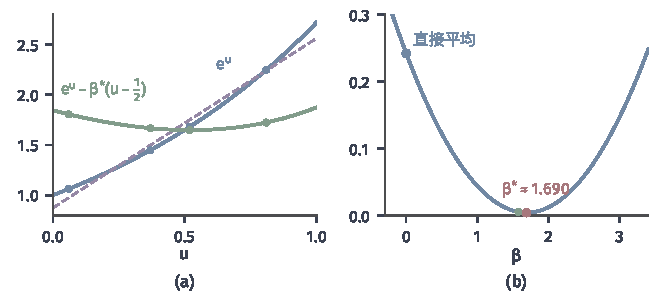
\includegraphics[width=112mm]{figures/07-probability/08-sampling-and-integration/matplotlib/vr-control-variate/figure.pdf}
 \caption{以$h(U)=U$为控制变量计算$\int_0^1\mathrm{e}^{u}\,\mathrm{d}u$。(a)蓝线为$\mathrm{e}^{u}$，紫色虚线为$I+\beta^{*}(u-\tfrac12)$，绿线为$\mathrm{e}^{u}-\beta^{*}(u-\tfrac12)$；圆点标出$u=0.37,0.81,0.06,0.52$处的值。(b)单样本方差$\sigma_f^2-2\beta\gamma+\beta^2/12$随$\beta$的变化：蓝点为直接平均，红点为$\beta^{*}$，绿点为由四个样本估计的$\hat{\beta}=1.577$。}
 \label{fig:vr-control-variate}
\end{BookInlineFigure}

\paragraph{系数由同一批样本估计}
实际中$\gamma$通常未知，$\beta^{*}$也就未知。最直接的办法是用同一批样本的样本协方差与样本方差估计它：
\begin{equation}
 \hat{\beta}=\frac{\sum_{i=1}^{n}\bigl(h(X_i)-\bar{h}\bigr)\bigl(f(X_i)-\bar{f}\bigr)}{\sum_{i=1}^{n}\bigl(h(X_i)-\bar{h}\bigr)^2} ,
 \label{eq:vr-cv-beta-hat}
\end{equation}
其中$\bar{f}$、$\bar{h}$是两列值的样本平均，再代入估计：
\[
 \hat{I}_n^{\mathrm{CV}}(\hat{\beta})=\bar{f}-\hat{\beta}(\bar{h}-\mu_h) .
\]这时减去的量$\hat{\beta}(\bar{h}-\mu_h)$是两个随机量的乘积，它的期望一般不为零：
\[
 \mathbb{E}\bigl[\hat{I}_n^{\mathrm{CV}}(\hat{\beta})\bigr]-I=-\mathbb{E}\bigl[\hat{\beta}(\bar{h}-\mu_h)\bigr]=-\operatorname{Cov}(\hat{\beta},\bar{h}) .
\]
这一偏差通常与$1/n$同阶。

另一方面，
\[
 \hat{I}_n^{\mathrm{CV}}(\hat{\beta})-\hat{I}_n^{\mathrm{CV}}(\beta^{*})=-(\hat{\beta}-\beta^{*})(\bar{h}-\mu_h) ,
\]
两个因子都以$n^{-1/2}$的速度趋于零，乘积是更高阶的量。所以样本量大时，用$\hat{\beta}$与用$\beta^{*}$的渐近方差相同，有限样本则多出一个偏差。

下面用四个均匀随机数逐步演示：
\[
 u=0.37,\quad 0.81,\quad 0.06,\quad 0.52 .
\]
函数值为
\[
 \mathrm{e}^{u}=1.44773,\quad 2.24791,\quad 1.06184,\quad 1.68203 ,
\]
直接平均$\bar{f}=1.60988$，$\bar{h}=0.44$。样本协方差与样本方差（分母都取$3$）分别为$0.15382$与$0.09753$，于是$\hat{\beta}=1.5771$。代入得
\[
 \hat{I}_4^{\mathrm{CV}}(\hat{\beta})=1.60988-1.5771\times(0.44-0.5)=1.70450 .
\]
若用$\beta^{*}$，结果是$1.71130$；真值为$1.71828$。四个样本的$\bar{h}$偏小$0.06$，直接平均随之偏低；控制变量按斜率把这一偏低补了回来。

\paragraph{独立预估系数}
若想保留严格的无偏性，可以用一批与正式样本独立的预备样本估计系数，得到$\widetilde{\beta}$，再在正式计算中当作常数使用。给定$\widetilde{\beta}$，由定义~\ref{def:vr-control-variate}后的论证，条件期望为$I$，所以估计无偏。由全方差公式，它的方差是$\mathbb{E}[\sigma^2(\widetilde{\beta})]/n$，其中$\sigma^2(\beta)$是式~\eqref{eq:vr-cv-variance}的右边；由配方结果，
\[
 \mathbb{E}\bigl[\sigma^2(\widetilde{\beta})\bigr]=\sigma_f^2(1-\rho^2)+\sigma_h^2\,\mathbb{E}\bigl[(\widetilde{\beta}-\beta^{*})^2\bigr] .
\]
最后一项是系数估计不准的代价。预备样本和每个样本上$h$的求值都要计入成本；$h$本身昂贵时，即使$\rho^2$很大，相对效率也可能不高。

\subsection{条件期望降方差}
\label{sec:vr-conditioning}

第~\ref{chap:laws-of-large-numbers}章用随机投点估计过四分之一圆的面积：设$X$与$Y$独立，都服从$\operatorname{Unif}(0,1)$，点落在单位圆内的概率是
\[
 I=\mathbb{P}(X^2+Y^2\leq1)=\frac{\pi}{4} .
\]
直接平均的是示性值$f(X,Y)=\mathbf{1}_{\{X^2+Y^2\leq1\}}$，每个样本只回答“在圆内吗”，单样本方差是$\tfrac{\pi}{4}(1-\tfrac{\pi}{4})\approx0.1685$。可是一旦知道$X=x$，点落在圆内当且仅当$Y\leq\sqrt{1-x^2}$，这件事的概率可以直接写出：
\[
 g(x)=\mathbb{P}\bigl(Y\leq\sqrt{1-x^2}\bigr)=\sqrt{1-x^2} .
\]
那么$Y$就不必再抽了：只抽$X$，平均$g(X)$。

\begin{theorem}[条件期望不增加方差]
\label{thm:vr-conditioning}
设输入为$(X,Y)$，$\mathbb{E}[f(X,Y)^2]<\infty$，记$g(X)=\mathbb{E}[f(X,Y)\mid X]$。则
\begin{equation}
 \mathbb{E}[g(X)]=I,\qquad \operatorname{Var}\bigl(g(X)\bigr)=\operatorname{Var}\bigl(f(X,Y)\bigr)-\mathbb{E}\bigl[\operatorname{Var}\bigl(f(X,Y)\bigm|X\bigr)\bigr] .
 \label{eq:vr-conditioning}
\end{equation}
所以对独立且同分布的$X_1,\dots,X_n$，平均$g(X_i)$的方差不超过同样个数的独立$(X_i,Y_i)$上平均$f$的方差；等号当且仅当$\operatorname{Var}(f(X,Y)\mid X)=0$几乎必然成立。
\end{theorem}

\begin{proof}
第一式是全期望公式。第二式是第~\ref{chap:conditional-expectation}章的全方差公式移项：
\[
 \operatorname{Var}(f)=\mathbb{E}\bigl[\operatorname{Var}(f\mid X)\bigr]+\operatorname{Var}\bigl(\mathbb{E}[f\mid X]\bigr) .
\]
减去的一项非负，所以$\operatorname{Var}(g(X))\leq\operatorname{Var}(f)$。两种平均都是$n$个独立同分布项的平均，方差各除以$n$，大小关系保持。减去的项为零当且仅当条件方差几乎必然为零。
\end{proof}

这种做法称为\term{条件Monte Carlo}（conditional Monte Carlo）。按第~\ref{chap:conditional-expectation}章的说法，条件期望是按$X$分组后的组内平均：直接抽样时，每个样本在自己的组里随机取一个值；条件化以后，每个样本直接报出组内平均。全方差公式中被减去的$\mathbb{E}[\operatorname{Var}(f\mid X)]$正是组内的平均波动，它被精确地算掉了。

\paragraph{四分之一圆的数值}
条件化后的方差为
\[
 \operatorname{Var}\bigl(g(X)\bigr)=\mathbb{E}[1-X^2]-\Bigl(\frac{\pi}{4}\Bigr)^2=\frac23-\frac{\pi^2}{16}\approx0.04982 ,
\]
被消去的组内波动为$0.1685-0.0498=0.1187$，方差降为原来的$1/3.38$。用下面四个点逐步演示：
\[
 (x,y)=(0.37,0.23),\quad(0.81,0.68),\quad(0.06,0.45),\quad(0.52,0.91) .
\]
第二、四个点在圆外，直接平均给出$0.5$，对应$\pi\approx2.0$。条件化只用四个$x$，
\[
 g(x)=0.92903,\quad 0.58643,\quad 0.99820,\quad 0.85417 ,
\]
平均为$0.84196$，对应$\pi\approx3.37$。

\begin{BookInlineFigure}
 \centering
 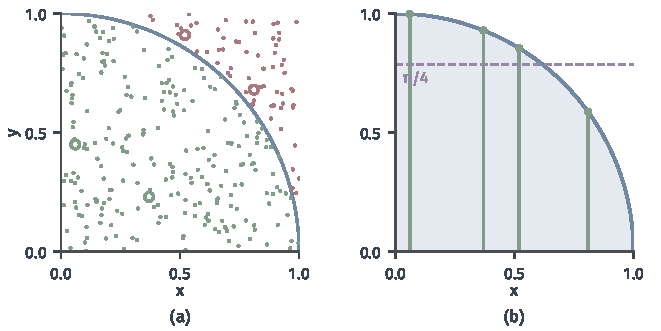
\includegraphics[width=112mm]{figures/07-probability/08-sampling-and-integration/matplotlib/vr-conditional/figure.pdf}
 \caption{用条件期望计算$\mathbb{P}(X^2+Y^2\leq1)=\pi/4$。(a)单位正方形中的$300$个随机点（种子2），圆内为绿色、圆外为红色，四个空心圆为正文的手算点；蓝线是四分之一圆周。(b)蓝线为$g(x)=\sqrt{1-x^2}$，绿色竖线是四个手算点的$x$处整条竖直切片在圆内的比例，紫色虚线为$\pi/4$。}
 \label{fig:vr-conditional}
\end{BookInlineFigure}

图~\ref{fig:vr-conditional}对比了两种计算。左图每个点只给出$0$或$1$；右图每个$x$给出整条竖直切片落在圆内的比例，样本之间的差别只来自$x$的不同。这里$g$只需一次开方，每个样本还少抽一个均匀数，成本不增反减。一般情形下，计算$g$可能需要一个积分，它的成本必须计入。

\paragraph{条件平均只能近似时}
若$g$没有闭式，需要用数值方法近似，定理~\ref{thm:vr-conditioning}的保证不能直接沿用，要看近似怎样做。

一种做法是确定性的求积。例如在每个$x$处，用$m$个等距中点$y_j=(j-\tfrac12)/m$数出满足$x^2+y_j^2\leq1$的比例，作为$g(x)$的近似$g_m(x)$。这个量不是$f$的条件期望，$\mathbb{E}[g_m(X)]\neq I$，产生一个不随$n$减小的偏差，需要像数值积分那样单独估计它的大小。

另一种做法是在每个$X_i$处再独立抽$m$个$Y_{i,1},\dots,Y_{i,m}$，平均$f(X_i,Y_{i,j})$。给定$X_i$时这$m$项独立同分布，所以内层平均的条件期望仍是$g(X_i)$，估计无偏。由全方差公式，内层平均的方差为
\[
 \operatorname{Var}\bigl(g(X)\bigr)+\frac{\mathbb{E}\bigl[\operatorname{Var}(f\mid X)\bigr]}{m} .
\]
$m=1$时回到直接平均，$m\to\infty$时趋于条件Monte Carlo，代价是每个外层样本做$m$次内层计算。四分之一圆中取$m=2$，方差为$0.0498+0.1187/2\approx0.1092$。


\section{改变抽样机制}
\label{sec:vr-change-mechanism}

前两节的方法都保持样本之间相互独立。独立有它的代价：$n$个独立均匀点可能挤在一处，也可能留下大片空白，每个区域分到多少样本完全由运气决定。本节放弃样本之间的独立，转而有计划地安排基础随机数：规定每个区域分到的点数，让点集整体上铺得均匀，或者让成对的输出朝相反或相同的方向变化。每个点的边缘分布仍然正确，所以估计仍然无偏；变化的是点与点之间的协方差。

\paragraph{把积分搬到单位立方体上}
设第~\ref{chap:sample-generation}章给出了一个可计算的生成映射$T:[0,1)^d\to\mathcal{X}$，使$\bm{U}\sim\operatorname{Unif}([0,1)^d)$时$T(\bm{U})\sim P$。记$F=f\circ T$，则
\begin{equation}
 I=\mathbb{E}_P[f(X)]=\int_{[0,1)^d}F(\bm{u})\,\mathrm{d}\bm{u} .
 \label{eq:vr-unit-cube}
\end{equation}
例如相关的高斯向量$\mathcal{N}(\bm{\mu},\bm{\Sigma})$可以取
\[
 T(\bm{u})=\bm{\mu}+\bm{L}\bigl(\Phi^{-1}(u_1),\dots,\Phi^{-1}(u_d)\bigr)^{\top} ,
\]
其中$\bm{L}$是协方差矩阵$\bm{\Sigma}$的Cholesky因子。点集的安排都在$\bm{u}$上进行，目标坐标之间的相关结构由$T$负责保留。这样，本节的方法只需要处理“单位立方体上的均匀点”这一种对象；代价是它们的效果取决于$F=f\circ T$的性质，而不仅是$f$的性质。

\subsection{分层采样}
\label{sec:vr-stratified}

用$8$个独立均匀点计算$\int_0^1\mathrm{e}^{u}\,\mathrm{d}u$，落在左半区间的点数服从$\operatorname{Bin}(8,1/2)$，有$7\%$的机会是$0$、$1$、$7$或$8$个。左半区间的函数值小、右半区间的大，点数的偶然多少直接变成估计的偏高或偏低。如果事先规定每个子区间各放几个点，这部分波动就消失了。

\begin{definition}[分层采样估计]
\label{def:vr-stratified}
把$\mathcal{X}$分成互不相交的集合$A_1,\dots,A_K$，称为层，设各层概率$p_k=P(A_k)>0$已知，并且能从条件分布$P(\cdot\mid A_k)$抽样。取正整数$n_1,\dots,n_K$，$\sum_kn_k=n$。各层内独立抽取$X_{k,1},\dots,X_{k,n_k}\sim P(\cdot\mid A_k)$，层间也相互独立。称
\begin{equation}
 \hat{I}^{\mathrm{st}}=\sum_{k=1}^{K}p_k\,\hat{\mu}_k,\qquad \hat{\mu}_k=\frac{1}{n_k}\sum_{i=1}^{n_k}f(X_{k,i})
 \label{eq:vr-stratified}
\end{equation}
为\term{分层采样}（stratified sampling）估计。
\end{definition}

记层内均值与层内方差为
\[
 \mu_k=\mathbb{E}[f(X)\mid X\in A_k],\qquad \sigma_k^2=\operatorname{Var}\bigl(f(X)\bigm|X\in A_k\bigr) .
\]

\begin{theorem}[分层估计的方差]
\label{thm:vr-stratified}
设$\mathbb{E}_P[f^2]<\infty$。则$\hat{I}^{\mathrm{st}}$无偏，且
\begin{equation}
 \operatorname{Var}\bigl(\hat{I}^{\mathrm{st}}\bigr)=\sum_{k=1}^{K}\frac{p_k^2\,\sigma_k^2}{n_k} .
 \label{eq:vr-stratified-variance}
\end{equation}
若按\term{比例分配}（proportional allocation）取$n_k=np_k$，则
\begin{equation}
 \operatorname{Var}\bigl(\hat{I}^{\mathrm{st}}\bigr)=\frac1n\sum_{k=1}^{K}p_k\sigma_k^2=\frac{\sigma^2}{n}-\frac1n\sum_{k=1}^{K}p_k(\mu_k-I)^2\leq\frac{\sigma^2}{n} .
 \label{eq:vr-proportional}
\end{equation}
\end{theorem}

\begin{proof}
由全概率公式，$\sum_kp_k\mu_k=I$；每个$\hat{\mu}_k$是$\mu_k$的无偏估计，所以$\hat{I}^{\mathrm{st}}$无偏。各层的样本相互独立，方差相加；$\hat{\mu}_k$的方差为$\sigma_k^2/n_k$，乘以系数的平方$p_k^2$即为第$k$层的贡献。

比例分配时代入$n_k=np_k$即得第一个等号。把层号$J$（$X\in A_J$）看成一个离散随机变量，由全方差公式，
\[
 \sigma^2=\mathbb{E}\bigl[\operatorname{Var}(f\mid J)\bigr]+\operatorname{Var}\bigl(\mathbb{E}[f\mid J]\bigr)=\sum_kp_k\sigma_k^2+\sum_kp_k(\mu_k-I)^2 ,
\]
移项得第二个等号。
\end{proof}

式~\eqref{eq:vr-proportional}说明比例分配的分层永远不比独立抽样差：它把总方差中的层间部分$\sum_kp_k(\mu_k-I)^2$整个去掉了。这一部分正是“各层分到多少点由运气决定”造成的波动。层分得越细、层均值差别越大，去掉的越多。

\paragraph{考虑波动与成本的分配}
比例分配没有利用各层的波动大小。设第$k$层每个样本的成本为$c_k$，总预算为$\sum_kc_kn_k=C$，在式~\eqref{eq:vr-stratified-variance}中选$n_k$。暂时允许$n_k$取正实数，由Cauchy--Schwarz不等式，
\[
 \Bigl(\sum_kp_k\sigma_k\sqrt{c_k}\Bigr)^2=\Bigl(\sum_k\frac{p_k\sigma_k}{\sqrt{n_k}}\cdot\sqrt{c_kn_k}\Bigr)^2\leq\Bigl(\sum_k\frac{p_k^2\sigma_k^2}{n_k}\Bigr)\Bigl(\sum_kc_kn_k\Bigr) .
\]
右边第二个因子是$C$，所以方差不小于$(\sum_kp_k\sigma_k\sqrt{c_k})^2/C$。等号当且仅当两个因子成比例，即
\begin{equation}
 n_k\propto\frac{p_k\sigma_k}{\sqrt{c_k}},\qquad \operatorname{Var}\bigl(\hat{I}^{\mathrm{st}}\bigr)_{\min}=\frac{\bigl(\sum_kp_k\sigma_k\sqrt{c_k}\bigr)^2}{C} .
 \label{eq:vr-neyman}
\end{equation}
波动大的层多放点，昂贵的层少放点。各层成本相同时$n_k\propto p_k\sigma_k$，称为\term{Neyman分配}（Neyman allocation）。实际的$n_k$要取整；若还要在层内估计方差，每层至少需要两个点。

\paragraph{例子：四层计算$\mathrm{e}-1$}
把$[0,1)$等分为四层，$p_k=1/4$。在宽为$1/4$的区间$[a,a+\tfrac14)$上，层均值与层内方差可以直接积分：
\[
 \mu_k=4\bigl(\mathrm{e}^{a+1/4}-\mathrm{e}^{a}\bigr),\qquad \sigma_k^2=2\bigl(\mathrm{e}^{2a+1/2}-\mathrm{e}^{2a}\bigr)-\mu_k^2 .
\]
四层的结果为
\[
 \begin{array}{lcccc}
  \text{层} & [0,\tfrac14) & [\tfrac14,\tfrac12) & [\tfrac12,\tfrac34) & [\tfrac34,1)\\
  \mu_k & 1.1361 & 1.4588 & 1.8731 & 2.4051\\
  \sigma_k & 0.0819 & 0.1052 & 0.1351 & 0.1735
 \end{array}
\]
取$n=8$，比例分配每层$2$个点，由式~\eqref{eq:vr-proportional}，
\[
 \operatorname{Var}\bigl(\hat{I}^{\mathrm{st}}\bigr)=\frac18\cdot\frac14\sum_k\sigma_k^2\approx0.002067 ,
\]
而$8$个独立点的方差为$0.24204/8\approx0.03025$，降为$1/14.6$。Neyman分配按$\sigma_k$的比例给出$n_k\approx1.32,1.70,2.18,2.80$，方差降到$0.001920$；取整为$1,2,2,3$时为$0.001963$，但第一层只有一个点，无法估计它的层内方差。这里各层波动相差不到三倍，最优分配只比比例分配好$7\%$。

下面用八个层内均匀数演示比例分配的计算，第$k$层的点取$u=(k-1+v)/4$：
\[
 v=0.37,\ 0.81\ \big|\ 0.06,\ 0.52\ \big|\ 0.23,\ 0.68\ \big|\ 0.45,\ 0.91 .
\]
得到的八个点依次为
\[
 u=0.0925,\ 0.2025,\ 0.265,\ 0.38,\ 0.5575,\ 0.67,\ 0.8625,\ 0.9775 .
\]
层均值的估计是每层两个$\mathrm{e}^{u}$的平均，再按$p_k=1/4$加权；因为比例分配，这等于八个函数值的普通平均：
\[
 \hat{I}^{\mathrm{st}}=\frac18\bigl(1.0969+1.2245+\cdots+2.6578\bigr)=1.7268 .
\]
真值为$1.7183$。

\begin{BookInlineFigure}
 \centering
 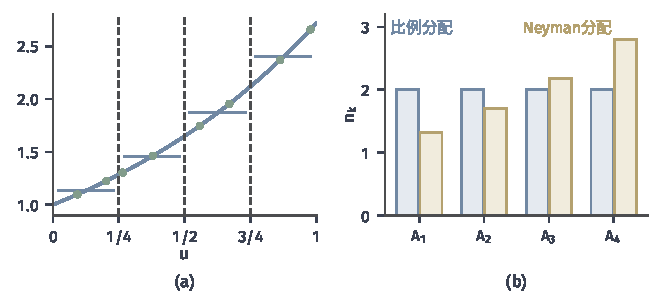
\includegraphics[width=112mm]{figures/07-probability/08-sampling-and-integration/matplotlib/vr-stratified/figure.pdf}
 \caption{四层分层采样计算$\int_0^1\mathrm{e}^{u}\,\mathrm{d}u$。(a)蓝线为$\mathrm{e}^{u}$，虚线为层的边界，蓝色短横线为层均值$\mu_k$，绿点为每层两个样本（$v$见正文）。(b)$n=8$时的样本分配：蓝色为比例分配$n_k=2$，黄色为Neyman分配$n_k\propto\sigma_k$。}
 \label{fig:vr-stratified}
\end{BookInlineFigure}

\paragraph{层越细越好，但维数会让层数爆炸}
图~\ref{fig:vr-stratified}(a)中，层内的函数几乎是直线，层内波动远小于整体波动。把$[0,1)$等分成$n$层、每层一个点，式~\eqref{eq:vr-stratified-variance}成为$n^{-2}\sum_k\sigma_k^2$。若$\lvert F'\rvert\leq L$，宽为$1/n$的层上$F$的取值范围不超过$L/n$，层内方差不超过$(L/n)^2/4$，于是
\[
 \operatorname{Var}\bigl(\hat{I}^{\mathrm{st}}\bigr)\leq\frac{1}{n^2}\cdot n\cdot\frac{L^2}{4n^2}=\frac{L^2}{4n^3} .
\]
方差按$n^{-3}$而非$n^{-1}$下降。到了$d$维，把每个坐标分成$m$段需要$m^d$个层，$d=10$、$m=2$就已经是$1024$层，每层至少一个点；预算不足$m^d$时，联合分层根本无法实施。

\paragraph{层的概率与分配不能由同一批数据随意决定}
定理~\ref{thm:vr-stratified}假设$p_k$已知、$n_k$事先固定。若$p_k$本身要从样本估计，估计量就变成两个随机量的组合，偏差和方差都要重新推导。若$n_k$按一次独立的试运行估计的$\sigma_k$确定，那么给定试运行结果，分配是固定的，定理的结论在条件意义下仍然成立；若边抽样边根据已抽到的值调整$n_k$，各层的样本数依赖于样本本身，式~\eqref{eq:vr-stratified-variance}不能直接套用，需要另行分析。

\subsection{拉丁超立方采样}
\label{sec:vr-lhs}

联合分层在高维失效，但退一步，可以只要求每个坐标各自分层：$n$个点投影到任何一根坐标轴上，都恰好在$n$个等长小区间中各占一个。这样，无论维数多大，$n$个点就够了。

\begin{definition}[拉丁超立方设计]
\label{def:vr-lhs}
给定点数$n$与维数$d$。取$d$个相互独立、在$\{1,\dots,n\}$的全部排列上均匀分布的随机排列$\pi_1,\dots,\pi_d$，再取与它们独立的$V_{i,j}\sim\operatorname{Unif}(0,1)$，$i=1,\dots,n$，$j=1,\dots,d$，全部相互独立。令
\begin{equation}
 U_{i,j}=\frac{\pi_j(i)-1+V_{i,j}}{n},\qquad \bm{U}_i=(U_{i,1},\dots,U_{i,d}) ,
 \label{eq:vr-lhs}
\end{equation}
用
\begin{equation}
 \hat{I}^{\mathrm{LHS}}=\frac1n\sum_{i=1}^{n}F(\bm{U}_i)
 \label{eq:vr-lhs-estimator}
\end{equation}
估计式~\eqref{eq:vr-unit-cube}的积分。
\end{definition}

第$i$个点的第$j$个坐标落在第$\pi_j(i)$层，层内位置由$V_{i,j}$决定。因为$\pi_j$是排列，第$j$个坐标的$n$个值恰好每层一个。这种设计称为拉丁超立方采样（Latin hypercube sampling，LHS），也叫\term{拉丁超立方抽样}。

\begin{theorem}[拉丁超立方的无偏性]
\label{thm:vr-lhs-unbiased}
在定义~\ref{def:vr-lhs}中，每个$\bm{U}_i$都服从$\operatorname{Unif}([0,1)^d)$。所以对可积的$F$，$\mathbb{E}[\hat{I}^{\mathrm{LHS}}]=I$。
\end{theorem}

\begin{proof}
固定$i$与$j$。均匀随机排列下$\pi_j(i)$在$\{1,\dots,n\}$上均匀分布，且与$V_{i,j}$独立。对$t\in[0,1]$，按层号分解，
\[
 \begin{aligned}
 \mathbb{P}(U_{i,j}\leq t)&=\sum_{k=1}^{n}\frac1n\,\mathbb{P}\Bigl(\frac{k-1+V_{i,j}}{n}\leq t\Bigr)\\
 &=\sum_{k=1}^{n}\frac1n\min\bigl\{1,\max\{0,nt-k+1\}\bigr\}=t .
 \end{aligned}
\]
最后一步中，$t$所在层之前的各层贡献$1/n$，$t$所在层贡献其中的一部分，之后的各层贡献$0$。不同的$j$用的是相互独立的$(\pi_j,V_{1,j},\dots,V_{n,j})$，所以$U_{i,1},\dots,U_{i,d}$相互独立，$\bm{U}_i$在立方体上均匀。对$n$个点的$F$值取期望并平均，得到无偏性。
\end{proof}

\paragraph{二维四点}
取$n=4$，$d=2$，两个排列与层内位置为
\[
 \pi_1=(2,4,1,3),\qquad \pi_2=(1,3,2,4) ,
\]
\[
 V_{:,1}=(0.37,0.81,0.06,0.52),\qquad V_{:,2}=(0.23,0.68,0.45,0.91) .
\]
由式~\eqref{eq:vr-lhs}，第一个点为
\[
 \bm{U}_1=\Bigl(\frac{1+0.37}{4},\ \frac{0+0.23}{4}\Bigr)=(0.3425,0.0575) .
\]
同样得到
\[
 \bm{U}_2=(0.9525,0.67),\qquad \bm{U}_3=(0.015,0.3625),\qquad \bm{U}_4=(0.63,0.9775) .
\]
图~\ref{fig:vr-lhs-points}(a)把单位正方形分成$4\times4$个格子：每行、每列恰好一个点，但$16$个格子只占了$4$个。逐维覆盖不等于覆盖全部坐标组合。图(b)是另一种同样合法的设计，两个排列都取恒等排列，四个点全落在对角线的格子里，坐标之间几乎完全相关。这种设计出现的概率是$1/4!$，它提醒我们：拉丁超立方只控制每个坐标的投影，不控制点在平面上的整体分布。

\begin{BookInlineFigure}
 \centering
 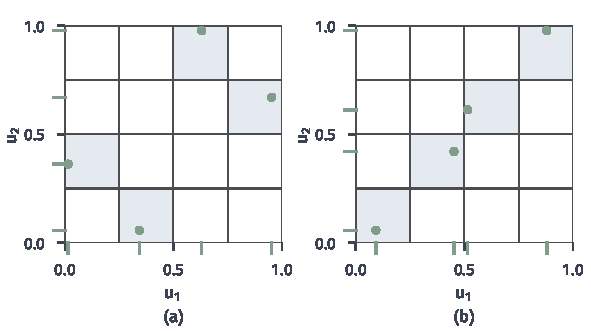
\includegraphics[width=100mm]{figures/07-probability/08-sampling-and-integration/matplotlib/vr-lhs-points/figure.pdf}
 \caption{$n=4$、$d=2$的拉丁超立方设计。灰线把正方形分成$4\times4$格，浅蓝格子含有一个点，坐标轴旁的绿色短线是点在各坐标上的投影。(a)$\pi_1=(2,4,1,3)$，$\pi_2=(1,3,2,4)$；(b)两个排列都是恒等排列。两者的$V$相同，见正文。}
 \label{fig:vr-lhs-points}
\end{BookInlineFigure}

对$F(\bm{u})=\mathrm{e}^{u_1}+\mathrm{e}^{u_2}$，真值$2(\mathrm{e}-1)=3.4366$。图(a)的四个点给出两列函数值的平均$1.7233$与$1.7770$，估计为$3.5004$。

\paragraph{可加函数：每个坐标都得到分层的好处}
先看$F$可以写成各坐标函数之和的情形。

\begin{theorem}[可加函数的拉丁超立方方差]
\label{thm:vr-lhs-additive}
设$F(\bm{u})=c+\sum_{j=1}^{d}g_j(u_j)$，各$g_j(U)$平方可积。记$\sigma_{j,k}^2$为$g_j(V)$在$V\sim\operatorname{Unif}([\tfrac{k-1}{n},\tfrac{k}{n}))$下的方差。则
\begin{equation}
 \operatorname{Var}\bigl(\hat{I}^{\mathrm{LHS}}\bigr)=\frac{1}{n^2}\sum_{j=1}^{d}\sum_{k=1}^{n}\sigma_{j,k}^2\leq\frac1n\sum_{j=1}^{d}\operatorname{Var}\bigl(g_j(U)\bigr) .
 \label{eq:vr-lhs-additive}
\end{equation}
\end{theorem}

\begin{proof}
估计量拆成$c+\sum_jT_j$，其中$T_j=\frac1n\sum_ig_j(U_{i,j})$只依赖第$j$列。第$j$列的$n$个值恰好每层一个，层内位置独立均匀，所以$T_j$正是每层一个点、$p_k=1/n$的分层估计，由式~\eqref{eq:vr-stratified-variance}，它的方差为$n^{-2}\sum_k\sigma_{j,k}^2$。不同列由相互独立的排列与层内位置生成，$T_1,\dots,T_d$相互独立，方差相加，得到等式。不等式是式~\eqref{eq:vr-proportional}对每一列的应用。
\end{proof}

对$F=\mathrm{e}^{u_1}+\mathrm{e}^{u_2}$，独立抽样的单点方差是$2\times0.24204$，而由上一小节的论证，式~\eqref{eq:vr-lhs-additive}按$n^{-3}$下降。图~\ref{fig:vr-lhs-variance}中绿线是比值$n\operatorname{Var}(\hat{I}^{\mathrm{LHS}})/\sigma^2$，它以$n^{-2}$的速度趋于零。

\paragraph{交互项：可能比独立抽样更差}
再看一个没有任何可加部分的函数。令$s(t)=1$（$t\geq\tfrac12$）或$-1$（$t<\tfrac12$），
\[
 F(\bm{u})=s(u_1)\,s(u_2) .
\]
$I=0$，$\sigma^2=1$，独立抽样的方差为$1/n$。设$n$为偶数，则第一个坐标落在下半区间$[0,\tfrac12)$的点恰有$n/2$个，第二个坐标也是。记$N$为两个坐标都在下半区间的点数。由$\pi_2$与$\pi_1$独立，第二个坐标落在下半区间的那些点是从$n$个点中均匀抽取的$n/2$个，所以$N$服从超几何分布$\operatorname{Hyp}(n,n/2,n/2)$。四类点的个数分别为
\[
 \text{下下}=N,\qquad \text{下上}=\text{上下}=\frac n2-N,\qquad \text{上上}=N .
\]

$F$在下下与上上处为$1$，其余为$-1$，于是
\[
 \hat{I}^{\mathrm{LHS}}=\frac{2N-2(n/2-N)}{n}=\frac{4N-n}{n} .
\]
由第~\ref{chap:common-distributions}章超几何分布的方差，
\[
 \operatorname{Var}(N)=\frac n2\cdot\frac12\cdot\frac12\cdot\frac{n-n/2}{n-1}=\frac{n^2}{16(n-1)} .
\]
所以
\begin{equation}
 \operatorname{Var}\bigl(\hat{I}^{\mathrm{LHS}}\bigr)=\frac{16}{n^2}\operatorname{Var}(N)=\frac{1}{n-1}>\frac1n .
 \label{eq:vr-lhs-interaction}
\end{equation}
$n=2$时方差为$1$，是独立抽样$1/2$的两倍：两点必然一个在左下或右上、另一个在相反的角，两个函数值相同，等于只抽了一个点。

\begin{BookInlineFigure}
 \centering
 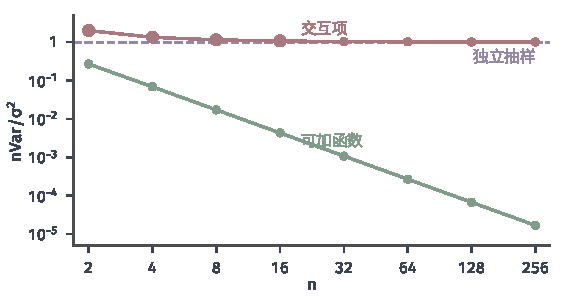
\includegraphics[width=96mm]{figures/07-probability/08-sampling-and-integration/matplotlib/vr-lhs-variance/figure.pdf}
 \caption{拉丁超立方的方差与独立抽样之比$n\operatorname{Var}(\hat{I}^{\mathrm{LHS}})/\sigma^2$，双对数坐标，$n$为偶数。绿线为可加函数$\mathrm{e}^{u_1}+\mathrm{e}^{u_2}$，按式~\eqref{eq:vr-lhs-additive}精确计算；红线为交互函数$s(u_1)s(u_2)$的精确值$n/(n-1)$，空心圆是$2\times10^{4}$次模拟（种子8）；紫色虚线为独立抽样。}
 \label{fig:vr-lhs-variance}
\end{BookInlineFigure}

\paragraph{一般函数}
一般的平方可积$F$可以分解为常数、各坐标的主效应$g_j(u_j)=\mathbb{E}[F(\bm{U})\mid U_j=u_j]-I$和剩下的交互部分。已知的结论是：拉丁超立方的方差等于$\sigma^2/n$减去$\frac1n\sum_j\operatorname{Var}(g_j(U_j))$，再加一个比$1/n$高阶的项；并且对任何平方可积的$F$和$n\geq2$，方差不超过$\sigma^2/(n-1)$。前者说明它去掉的正是主效应，后者说明它最多比独立抽样差一个因子$n/(n-1)$，式~\eqref{eq:vr-lhs-interaction}恰好达到这个上界。这两个结论的证明需要对排列做较长的组合计算，这里只用它们解释图~\ref{fig:vr-lhs-variance}：$F$越接近可加，拉丁超立方越有效；$F$以交互为主时，它几乎没有好处，有限样本下还可能略差。

\paragraph{误差怎样估计}
同一设计中的$n$个点不独立，它们的$F$值的样本方差除以$n$不是$\operatorname{Var}(\hat{I}^{\mathrm{LHS}})$的估计。正确的做法是第~\ref{chap:monte-carlo-integration-error}章的整组重复：独立生成$R$个设计，得到$R$个估计$Q_1,\dots,Q_R$，总平均$\bar{Q}$的方差用$s_Q^2/R$估计，$s_Q^2$是$Q_r$的样本方差。

\subsection{随机化准蒙特卡洛}
\label{sec:vr-rqmc}

分层与拉丁超立方都只控制点在若干固定格子中的个数。更直接的想法是：让点集在任何位置、任何尺度上都铺得均匀。先要有一个衡量“铺得均不均匀”的量。

对$\bm{b}\in[0,1]^d$，考虑以原点为一角的盒子$[\bm{0},\bm{b})=[0,b_1)\times\cdots\times[0,b_d)$。点集$\bm{a}_1,\dots,\bm{a}_n$均匀时，落进盒子的点的比例应当接近盒子的体积。

\begin{definition}[星差异]
\label{def:vr-star-discrepancy}
点集$\bm{a}_1,\dots,\bm{a}_n\in[0,1)^d$的\term{星差异}（star discrepancy）为
\begin{equation}
 D_n^{*}=\sup_{\bm{b}\in[0,1]^d}\Bigl\lvert\frac{\#\{i:\bm{a}_i\in[\bm{0},\bm{b})\}}{n}-\prod_{j=1}^{d}b_j\Bigr\rvert .
 \label{eq:vr-star-discrepancy}
\end{equation}
\end{definition}

一维时容易算。等距点$a_i=(i-1)/n$在$b$略大于$(i-1)/n$时，盒子里有$i$个点而长度只有约$(i-1)/n$，差$1/n$，所以$D_n^{*}=1/n$。把它们右移半格成$a_i=(i-\tfrac12)/n$，最大偏差减半为$1/(2n)$。$n=4$时，前者为$1/4$，后者为$1/8$。

图~\ref{fig:vr-discrepancy}比较了二维的两组$13$个点。独立均匀点（种子4）中，盒子$[0,0.607)\times[0,1)$的体积为$0.607$，却只含$3$个点，比例$0.231$，差$0.377$，这就是它的星差异。右图是一种规则构造：
\[
 \bm{a}_i=\Bigl(\frac{i-1}{13},\ \Bigl\{\frac{8(i-1)}{13}\Bigr\}\Bigr),\qquad i=1,\dots,13 ,
\]
其中$\{x\}=x-\lfloor x\rfloor$表示小数部分。它的星差异为$0.166$，由盒子$[0,0.538]\times[0,0.692]$达到：盒子连同边界上的点共$7$个，比例$0.538$，体积$0.373$。

\begin{BookInlineFigure}
 \centering
 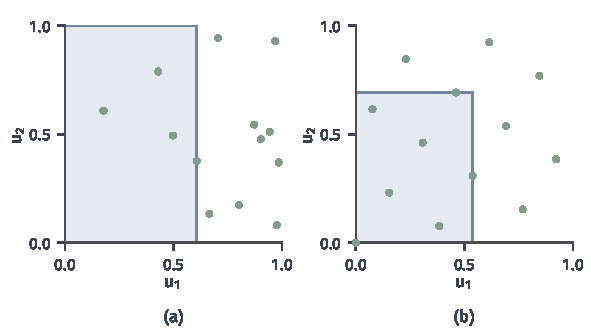
\includegraphics[width=100mm]{figures/07-probability/08-sampling-and-integration/matplotlib/vr-discrepancy/figure.pdf}
 \caption{$13$个点的星差异。浅蓝矩形是取到式~\eqref{eq:vr-star-discrepancy}中上确界的锚定盒子。(a)独立均匀点（种子4），盒子$[0,0.607)\times[0,1)$内只有$3$个点，$D_{13}^{*}=0.377$；(b)格点$((i-1)/13,\{8(i-1)/13\})$，盒子$[0,0.538]\times[0,0.692]$连同边界含$7$个点，$D_{13}^{*}=0.166$。}
 \label{fig:vr-discrepancy}
\end{BookInlineFigure}

\paragraph{确定性点集的积分误差}
用一个确定的点集代替随机样本，直接平均各点上的函数值，称为\term{准蒙特卡洛}（quasi-Monte Carlo）方法。它的误差由一个把函数与点集分开的不等式控制，称为\term{Koksma--Hlawka不等式}（Koksma--Hlawka inequality）：
\begin{equation}
 \Bigl\lvert\frac1n\sum_{i=1}^{n}F(\bm{a}_i)-\int_{[0,1)^d}F(\bm{u})\,\mathrm{d}\bm{u}\Bigr\rvert\leq V_{\mathrm{HK}}(F)\,D_n^{*} ,
 \label{eq:vr-koksma-hlawka}
\end{equation}
其中$V_{\mathrm{HK}}(F)$是$F$在Hardy--Krause意义下的变差，一维时就是$F$的全变差。证明需要多元的分部求和与变差的定义，篇幅较长。它的含义是：误差等于函数的起伏程度乘以点集的不均匀程度。一维的情形可以直接体会：$F$单调时，误差不超过$F$的总升降乘以$D_n^{*}$。

已有构造能使$D_n^{*}$随$n$按$(\ln n)^d/n$的阶下降，这样的点集称为\term{低差异点集}（low-discrepancy point set）；独立均匀点的星差异只按$n^{-1/2}$的阶下降。于是对$V_{\mathrm{HK}}(F)<\infty$的函数，准蒙特卡洛的误差在$n$很大时比$n^{-1/2}$小得多。但式~\eqref{eq:vr-koksma-hlawka}有三个局限：$V_{\mathrm{HK}}(F)$对无界函数和边界倾斜的示性函数是无穷；两个因子都难以计算，界本身不能用来报告误差；点集是确定的，算一次得到一个数，没有任何关于误差大小的信息。

\paragraph{加入随机性}
解决最后一个问题的办法是把整组点随机化：施加一个随机变换，使每个点单独看都服从均匀分布，而点集的均匀结构保持不变。这样得到的方法称为\term{随机化准蒙特卡洛}（randomized quasi-Monte Carlo，RQMC）。每个点均匀，保证估计无偏；整组独立重复若干次，就可以用第~\ref{chap:monte-carlo-integration-error}章的组间方差估计误差。下面讨论最简单的随机化，以及误差衰减的速度由什么决定。

\subsubsection{随机移位}
\label{sec:vr-random-shift}

把单位立方体的相对两面粘起来，它就成为一个环面：从右边出去的点从左边回来。在环面上整体平移一个点集，点与点之间的相对位置不变。

\begin{definition}[随机移位]
\label{def:vr-random-shift}
给定点集$\bm{a}_1,\dots,\bm{a}_n\in[0,1)^d$，取$\bm{\Delta}\sim\operatorname{Unif}([0,1)^d)$，令
\begin{equation}
 \bm{U}_i=(\bm{a}_i+\bm{\Delta})\bmod1,\qquad i=1,\dots,n ,
 \label{eq:vr-random-shift}
\end{equation}
其中$\bmod1$逐坐标取小数部分。所有点共用同一个$\bm{\Delta}$。称$Q=\frac1n\sum_iF(\bm{U}_i)$为\term{随机移位}（random shift）估计。
\end{definition}

例如$a=0.75$、$\Delta=0.37$时，$a+\Delta=1.12$，取小数部分得$0.12$：点从右端越过$1$后回到左端。图~\ref{fig:vr-random-shift}把上面的$13$点格点整体平移$\bm{\Delta}=(0.37,0.81)$：左图中平移后的点散在$[0,2)^2$的四块单位正方形里，右图把它们按$\bmod1$折回$[0,1)^2$，得到的仍是同一个格点结构，只是整体挪了位置。

\begin{BookInlineFigure}
 \centering
 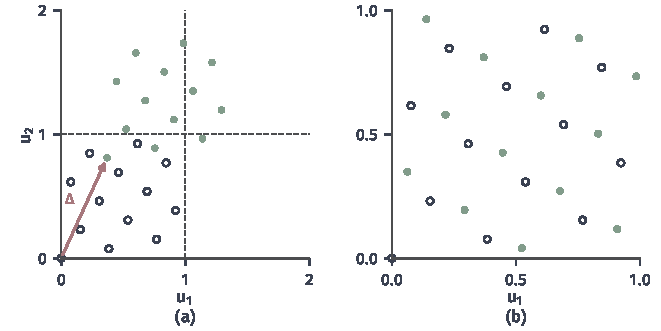
\includegraphics[width=112mm]{figures/07-probability/08-sampling-and-integration/matplotlib/vr-random-shift/figure.pdf}
 \caption{对$13$点格点的随机移位，$\bm{\Delta}=(0.37,0.81)$。空心圆为原格点，红色箭头为$\bm{\Delta}$。(a)平移后的点$\bm{a}_i+\bm{\Delta}$（绿色），虚线把$[0,2)^2$分成四块单位正方形；(b)逐坐标取小数部分后的$\bm{U}_i$（绿色）。}
 \label{fig:vr-random-shift}
\end{BookInlineFigure}

\begin{theorem}[随机移位的无偏性与方差]
\label{thm:vr-random-shift}
在定义~\ref{def:vr-random-shift}中，每个$\bm{U}_i$都服从$\operatorname{Unif}([0,1)^d)$，所以对可积的$F$，$\mathbb{E}[Q]=I$。若$F$平方可积，记其Fourier系数与点集的指数和为
\begin{equation}
 \begin{gathered}
 \hat{F}(\bm{h})=\int_{[0,1)^d}F(\bm{u})\mathrm{e}^{-2\pi\mathrm{i}\langle\bm{h},\bm{u}\rangle}\,\mathrm{d}\bm{u},\\
 S(\bm{h})=\frac1n\sum_{i=1}^{n}\mathrm{e}^{2\pi\mathrm{i}\langle\bm{h},\bm{a}_i\rangle},\qquad \bm{h}\in\mathbb{Z}^d ,
 \end{gathered}
 \label{eq:vr-fourier-sum}
\end{equation}
则
\begin{equation}
 \operatorname{Var}(Q)=\sum_{\bm{h}\neq\bm{0}}\bigl\lvert\hat{F}(\bm{h})\bigr\rvert^2\bigl\lvert S(\bm{h})\bigr\rvert^2 .
 \label{eq:vr-shift-variance}
\end{equation}
\end{theorem}

\begin{proof}
先证均匀性。一维时，固定$a\in[0,1)$，映射$\delta\mapsto(a+\delta)\bmod1$把$[0,1-a)$平移$a$得到$[a,1)$，把$[1-a,1)$平移$a-1$得到$[0,a)$，两段平移都保持长度，所以它把$[0,1)$上的均匀分布映成均匀分布。$d$维时$\bm{\Delta}$的各坐标独立，$\bm{U}_i$的各坐标也就独立且各自均匀。对$n$个点平均并取期望，得到无偏性。

再算方差。把$Q$看成$\bm{\Delta}$的函数：
\[
 Q(\bm{\Delta})=\frac1n\sum_{i=1}^{n}F\bigl((\bm{a}_i+\bm{\Delta})\bmod1\bigr) .
\]由平移保持均匀分布，每一项与$F$有相同的$L^2$范数，所以$Q$平方可积。

计算$Q$的Fourier系数时，对第$i$项作变量替换$\bm{v}=(\bm{a}_i+\bm{\Delta})\bmod1$，这一替换保持均匀测度。因为$\bm{h}$是整数向量，取小数部分不改变指数：
\[
 \mathrm{e}^{-2\pi\mathrm{i}\langle\bm{h},\bm{\Delta}\rangle}=\mathrm{e}^{-2\pi\mathrm{i}\langle\bm{h},\bm{v}\rangle}\,\mathrm{e}^{2\pi\mathrm{i}\langle\bm{h},\bm{a}_i\rangle} .
\]
于是
\[
 \hat{Q}(\bm{h})=\frac1n\sum_{i=1}^{n}\mathrm{e}^{2\pi\mathrm{i}\langle\bm{h},\bm{a}_i\rangle}\int_{[0,1)^d}F(\bm{v})\mathrm{e}^{-2\pi\mathrm{i}\langle\bm{h},\bm{v}\rangle}\,\mathrm{d}\bm{v}=\hat{F}(\bm{h})\,S(\bm{h}) .
\]

函数族$\mathrm{e}^{2\pi\mathrm{i}\langle\bm{h},\bm{u}\rangle}$（$\bm{h}\in\mathbb{Z}^d$）是$L^2([0,1)^d)$的完备正交规范系（可参考\BookChapterRef{chap:fourier-transform}{卷四第14章“Fourier变换”}），由Parseval等式（可参考\BookChapterRef{chap:function-inner-product-spaces}{卷四第12章“内积空间”}），
\[
 \mathbb{E}\bigl[\lvert Q\rvert^2\bigr]=\sum_{\bm{h}\in\mathbb{Z}^d}\bigl\lvert\hat{F}(\bm{h})S(\bm{h})\bigr\rvert^2 .
\]
$\bm{h}=\bm{0}$一项是$\lvert\hat{F}(\bm{0})\rvert^2=I^2$，因为$S(\bm{0})=1$。减去$I^2$即得式~\eqref{eq:vr-shift-variance}。
\end{proof}

\paragraph{点集是一个频率滤波器}
把式~\eqref{eq:vr-shift-variance}与独立抽样比较。对$F$本身用Parseval等式，
\[
 \sigma^2=\sum_{\bm{h}\neq\bm{0}}\bigl\lvert\hat{F}(\bm{h})\bigr\rvert^2 ,
\]
所以独立抽样的方差$\sigma^2/n$相当于给每个频率都乘上$1/n$。随机移位则给频率$\bm{h}$乘上$\lvert S(\bm{h})\rvert^2$。好的点集让$S(\bm{h})$在低频处为零或很小，只在少数高频处较大；只要$F$的能量主要集中在低频，方差就远小于$\sigma^2/n$。

格点是最干净的例子。取整数向量$\bm{z}$，令$\bm{a}_i=\{(i-1)\bm{z}/n\}$（逐坐标取小数部分）。$S(\bm{h})$是$n$个单位根的平均：若$\langle\bm{h},\bm{z}\rangle$是$n$的倍数，每项都是$1$，$S(\bm{h})=1$；否则$\mathrm{e}^{2\pi\mathrm{i}\langle\bm{h},\bm{z}\rangle/n}\neq1$，等比数列求和得$S(\bm{h})=0$。于是
\begin{equation}
 \operatorname{Var}(Q)=\sum_{\bm{h}\neq\bm{0},\ \langle\bm{h},\bm{z}\rangle\equiv0\ (\mathrm{mod}\ n)}\bigl\lvert\hat{F}(\bm{h})\bigr\rvert^2 .
 \label{eq:vr-lattice-variance}
\end{equation}
图~\ref{fig:vr-discrepancy}(b)的点集就是$n=13$、$\bm{z}=(1,8)$的格点，这类规则称为\term{秩1格点规则}（rank-1 lattice rule）。

\paragraph{一维等距点}
$d=1$、$z=1$时，$a_i=(i-1)/n$，只有$h$为$n$的倍数时$S(h)=1$，式~\eqref{eq:vr-lattice-variance}成为$\sum_{m\neq0}\lvert\hat{F}(mn)\rvert^2$。对$F(u)=\mathrm{e}^{u}$，
\[
 \hat{F}(h)=\int_0^1\mathrm{e}^{(1-2\pi\mathrm{i}h)u}\,\mathrm{d}u=\frac{\mathrm{e}-1}{1-2\pi\mathrm{i}h},\qquad \bigl\lvert\hat{F}(h)\bigr\rvert^2=\frac{(\mathrm{e}-1)^2}{1+4\pi^2h^2} .
\]
于是
\[
 \operatorname{Var}(Q)=2(\mathrm{e}-1)^2\sum_{m=1}^{\infty}\frac{1}{1+4\pi^2m^2n^2}\approx\frac{2(\mathrm{e}-1)^2}{4\pi^2n^2}\cdot\frac{\pi^2}{6}=\frac{(\mathrm{e}-1)^2}{12n^2} ,
\]
近似一步用了$\sum_m1/m^2=\pi^2/6$并略去分母中的$1$。均方根误差约为$0.496/n$，而独立抽样是$0.492/\sqrt{n}$。$n=4$时级数的精确值为$\operatorname{Var}(Q)=0.01536$，独立抽样为$0.06051$；$n=64$时分别为$6.01\times10^{-5}$与$3.78\times10^{-3}$。

\paragraph{整组重复估计误差}
取$n=4$的等距点$a=(0,\tfrac14,\tfrac12,\tfrac34)$，独立做$R=3$次随机移位。下面用三个移位量逐步演示：
\[
 \Delta=0.37,\quad 0.81,\quad 0.23 .
\]
第一次移位的点为$0.37,0.62,0.87,0.12$，其余两次分别为$0.81,0.06,0.31,0.56$与$0.23,0.48,0.73,0.98$。三组的估计为
\[
 Q_1=1.7053,\quad Q_2=1.6060,\quad Q_3=1.9036 .
\]
总平均$\bar{Q}=1.7383$，三个值的样本标准差$s_Q=0.1515$，标准误差估计为$s_Q/\sqrt3=0.0875$。按上面的精确方差，$\bar{Q}$的真实标准差是$\sqrt{0.01536/3}=0.0716$；同样$12$次求值的独立抽样标准差是$\sqrt{0.24204/12}=0.142$。三次重复给出的标准误差本身很粗糙；要构造第~\ref{chap:monte-carlo-integration-error}章的渐近误差区间，需要重复次数$R$趋于无穷，组内点数$n$固定时少量重复不能提供覆盖保证。同一组内的$4$个点不独立，不能用它们的样本方差除以$4$代替组间方差。

\subsubsection{误差衰减的条件}
\label{sec:vr-rqmc-rates}

随机移位对任何可积的$F$都无偏，但误差缩小得多快，由式~\eqref{eq:vr-shift-variance}决定：要看$F$的Fourier系数在$S(\bm{h})$较大的那些频率上衰减得多快。系数的衰减速度又由$F$在环面上的光滑程度决定，这里的“光滑”包括把立方体首尾粘起来以后的连续性。下面用一维等距点比较三种函数。

\paragraph{光滑但不周期}
$F(u)=\mathrm{e}^{u}$在$[0,1)$内光滑，但$F(0)=1\neq\mathrm{e}=F(1^{-})$，粘成圆周后在原点有一个跳跃。跳跃使$\hat{F}(h)$只按$1/\lvert h\rvert$衰减，上面已经算出均方根误差按$n^{-1}$下降。

\paragraph{换一个生成映射}
帐篷映射$\tau(u)=1-\lvert2u-1\rvert$把$\operatorname{Unif}(0,1)$映成$\operatorname{Unif}(0,1)$：对$t\in[0,1]$，$\tau(u)\leq t$当且仅当$u\leq t/2$或$u\geq1-t/2$，概率为$t$。所以$\widetilde{F}=F\circ\tau$与$F$的积分相同，单点方差也相同，只是换了一个生成映射。$\widetilde{F}(0)=\widetilde{F}(1^{-})=F(0)$，粘起来后连续，只在$u=\tfrac12$和原点处有折角，Fourier系数按$1/h^2$衰减，均方根误差按$n^{-2}$下降。

\paragraph{生成映射制造的奇异}
设目标是Pareto分布，$\mathbb{P}(X>x)=x^{-3}$（$x\geq1$），要算$\mathbb{E}[X]=3/2$。被积函数$f(x)=x$再光滑不过，但逆分位数映射$T(u)=(1-u)^{-1/3}$在$u\to1$时趋于无穷，于是
\[
 F(u)=f\bigl(T(u)\bigr)=(1-u)^{-1/3} .
\]
$\int_0^1(1-u)^{-2/3}\,\mathrm{d}u=3<\infty$，$F$平方可积，单点方差为$3-\tfrac94=\tfrac34$。但它在$u=1$处无界，$V_{\mathrm{HK}}(F)=\infty$，Koksma--Hlawka不等式失效。奇点$(1-u)^{-1/3}$使$\hat{F}(h)$只按$\lvert h\rvert^{-2/3}$衰减，于是方差按$\sum_m(mn)^{-4/3}\propto n^{-4/3}$下降，均方根误差按$n^{-2/3}$下降：仍比独立抽样快，但远慢于$\mathrm{e}^{u}$。

图~\ref{fig:vr-rqmc-rates}把三种情形与独立抽样画在一起，纵轴是均方根误差除以单点标准差。四条线的斜率依次接近$-\tfrac12$、$-\tfrac23$、$-1$、$-2$。同一个点集、同样的随机化，误差速度相差悬殊，差别全在$F=f\circ T$。

\begin{BookInlineFigure}
 \centering
 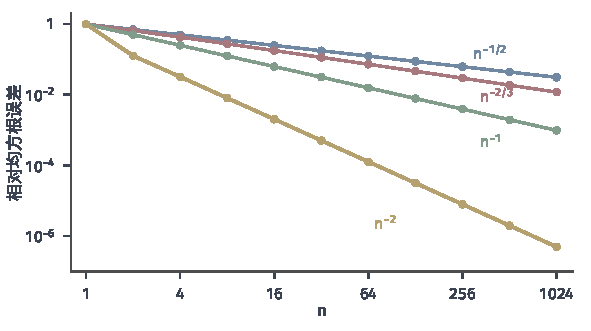
\includegraphics[width=100mm]{figures/07-probability/08-sampling-and-integration/matplotlib/vr-rqmc-rates/figure.pdf}
 \caption{一维等距点随机移位的相对均方根误差$\sqrt{\operatorname{Var}(Q)}/\sigma$，双对数坐标，由$\operatorname{Var}(Q)=n\int_0^{1/n}(Q(\Delta)-I)^2\,\mathrm{d}\Delta$数值积分得到。蓝线为独立抽样$n^{-1/2}$；绿线为$F(u)=\mathrm{e}^{u}$；黄线为帐篷映射后的$\mathrm{e}^{1-\lvert2u-1\rvert}$；红线为Pareto例子的$F(u)=(1-u)^{-1/3}$。}
 \label{fig:vr-rqmc-rates}
\end{BookInlineFigure}

\paragraph{点集与随机化方式}
高维时情况类似，但要同时看点集与随机化方式。格点配合随机移位，对在环面上光滑、Fourier系数衰减快的函数效果最好。另一大类低差异点集称为数字网，它的均匀结构是按二进制位定义的，普通的模$1$平移会破坏这种结构，需要配合按位的随机化，例如随机置乱。已知在被积函数足够光滑时，随机置乱的数字网的均方根误差可以接近$n^{-3/2}$的阶；这一结论的证明较长。无论哪种组合，更快的速度都只在相应的光滑条件下成立。

所以，不能只凭原函数$f$光滑，或者只凭点集差异小，就断言准蒙特卡洛会更准。要检查的是映射后的$F=f\circ T$：它在立方体边界上是否有界、粘起来后是否连续、是否有不沿坐标方向的间断。遇到不利的情形，可以像帐篷映射那样换一个生成映射，或者把奇异部分单独处理；无论效果如何，误差都用整组独立重复来估计。

\subsection{对偶变量}
\label{sec:vr-antithetic}

回到$\int_0^1\mathrm{e}^{u}\,\mathrm{d}u$。$U$与$1-U$都服从$\operatorname{Unif}(0,1)$，而且一个偏大时另一个必然偏小。把它们配成一对，$\mathrm{e}^{U}$偏高的那一次，$\mathrm{e}^{1-U}$就偏低，平均以后偏差部分抵消。

\begin{definition}[对偶变量估计]
\label{def:vr-antithetic}
设$n=2m$，$U_1,\dots,U_m$独立且都服从$\operatorname{Unif}(0,1)$。称
\begin{equation}
 \hat{I}^{\mathrm{anti}}=\frac1m\sum_{i=1}^{m}\frac{F(U_i)+F(1-U_i)}{2}
 \label{eq:vr-antithetic}
\end{equation}
为\term{对偶变量法}（antithetic variates）估计。它用了$n$次函数求值。
\end{definition}

每一对内两点的边缘分布都正确，所以估计无偏。记$\sigma^2=\operatorname{Var}(F(U))$，$\gamma=\operatorname{Cov}(F(U),F(1-U))$。一对的平均的方差为$(\sigma^2+\gamma)/2$，$m$对独立，所以
\begin{equation}
 \operatorname{Var}\bigl(\hat{I}^{\mathrm{anti}}\bigr)=\frac{\sigma^2+\gamma}{2m}=\frac{\sigma^2+\gamma}{n} .
 \label{eq:vr-antithetic-variance}
\end{equation}
同样$n$次求值的独立抽样方差是$\sigma^2/n$。两者相比，对偶变量严格更好当且仅当$\gamma<0$。

\begin{theorem}[单调函数的对偶协方差]
\label{thm:vr-antithetic-monotone}
设$F$在$(0,1)$上单调，$F(U)$平方可积。则$\operatorname{Cov}(F(U),F(1-U))\leq0$。
\end{theorem}

\begin{proof}
不妨设$F$不减。取与$U$独立同分布的$V$。若$U\geq V$，则$F(U)\geq F(V)$，同时$1-U\leq1-V$，$F(1-U)\leq F(1-V)$；$U<V$时两个不等号都反过来。所以
\[
 \bigl(F(U)-F(V)\bigr)\bigl(F(1-U)-F(1-V)\bigr)\leq0 .
\]
展开左边并取期望。由独立性与$1-V\sim\operatorname{Unif}(0,1)$，交叉项的期望都是$I^2$，于是期望等于$2\mathbb{E}[F(U)F(1-U)]-2I^2=2\gamma$，所以$\gamma\leq0$。
\end{proof}

\paragraph{例子与反例}
对$F(u)=\mathrm{e}^{u}$，$F(U)F(1-U)=\mathrm{e}$是常数，
\[
 \gamma=\mathrm{e}-(\mathrm{e}-1)^2\approx-0.23421 .
\]
由式~\eqref{eq:vr-antithetic-variance}，每次求值折合的方差为$\sigma^2+\gamma=0.24204-0.23421=0.00783$，相对效率约为$31$。用$u=0.37$与$0.81$各配一对：
\[
 \tfrac12(\mathrm{e}^{0.37}+\mathrm{e}^{0.63})=1.66267,\qquad \tfrac12(\mathrm{e}^{0.81}+\mathrm{e}^{0.19})=1.72858 ,
\]
平均$1.69563$。

反过来取关于$\tfrac12$对称的$F(u)=(u-\tfrac12)^2$，$I=1/12$。这时$F(1-U)=F(U)$，一对中的两个值完全相同，$\gamma=\sigma^2$，式~\eqref{eq:vr-antithetic-variance}给出$2\sigma^2/n$，是独立抽样的两倍：花了两次求值，只得到一个样本的信息。输入方向相反，本身不保证输出负相关。图~\ref{fig:vr-antithetic}对比了这两种情形。

\begin{BookInlineFigure}
 \centering
 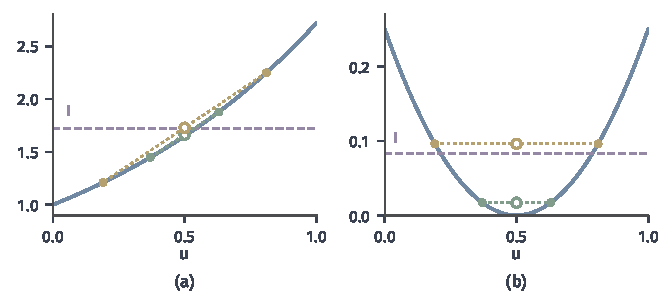
\includegraphics[width=112mm]{figures/07-probability/08-sampling-and-integration/matplotlib/vr-antithetic/figure.pdf}
 \caption{对偶对$(u,1-u)$，$u=0.37$（绿）与$u=0.81$（黄），实心点为两个函数值，$u=\tfrac12$处的空心圆为一对的平均，紫色虚线为积分值$I$。(a)单调的$\mathrm{e}^{u}$：一对的两个值分居$I$两侧，平均接近$I$；(b)对称的$(u-\tfrac12)^2$：一对的两个值相同，平均就是单个值。}
 \label{fig:vr-antithetic}
\end{BookInlineFigure}

\paragraph{奇偶分解}
两个例子可以统一起来。把$F$分成关于$\tfrac12$的偶部与奇部，
\[
 F_{\mathrm{e}}(u)=\frac{F(u)+F(1-u)}{2},\qquad F_{\mathrm{o}}(u)=\frac{F(u)-F(1-u)}{2} .
\]
一对的平均恰好是$F_{\mathrm{e}}(U)$，奇部被完全消去。$F_{\mathrm{e}}F_{\mathrm{o}}$关于$\tfrac12$是奇函数，积分为零，且$\mathbb{E}[F_{\mathrm{o}}(U)]=0$，所以$F_{\mathrm{e}}(U)$与$F_{\mathrm{o}}(U)$不相关，
\[
 \sigma^2=\operatorname{Var}\bigl(F_{\mathrm{e}}(U)\bigr)+\operatorname{Var}\bigl(F_{\mathrm{o}}(U)\bigr) .
\]
于是同样两次求值下，
\[
 \text{对偶一对的方差}=\operatorname{Var}(F_{\mathrm{e}}),\qquad \text{独立两点的方差}=\frac{\operatorname{Var}(F_{\mathrm{e}})+\operatorname{Var}(F_{\mathrm{o}})}{2} .
\]
对偶变量更好，当且仅当奇部的方差大于偶部的方差。单调函数以奇部为主，对称函数只有偶部。在$d$维中把$\bm{U}$换成$\bm{1}-\bm{U}$，对每个坐标都单调的$F$同样有$\gamma\leq0$，这一推广的证明要用到关于单调函数的关联不等式，篇幅较长；奇偶分解的判别对$d$维照样成立，论证与上面相同。

\subsection{共同随机数}
\label{sec:vr-crn}

另一类问题要比较两个方案。设方案A、B的输出分别为随机变量$A$与$B$，要估计期望差$\mathbb{E}[A]-\mathbb{E}[B]$。如果两个方案各自独立抽样，差的估计的方差是两者方差之和；但两个方案往往对同一种随机输入作出相似的反应，若让它们看到同一组随机输入，共同的波动就会在相减时抵消。

\paragraph{方差公式}
设$A=a(\bm{U})$，$B=b(\bm{U})$，$a(\bm{U})$与$b(\bm{U})$分别服从两个方案各自的输出分布。独立生成$\bm{U}_1,\dots,\bm{U}_n$，用
\[
 \hat{\Delta}=\frac1n\sum_{i=1}^{n}\bigl(a(\bm{U}_i)-b(\bm{U}_i)\bigr)
\]
估计$\mathbb{E}[A]-\mathbb{E}[B]$，这种做法称为\term{共同随机数}（common random numbers）。二阶矩有限时，
\begin{equation}
 n\operatorname{Var}(\hat{\Delta})=\operatorname{Var}(A)+\operatorname{Var}(B)-2\operatorname{Cov}(A,B) .
 \label{eq:vr-crn}
\end{equation}
两方案各用$n$个独立输入时，同样$2n$次求值得到的是$\operatorname{Var}(A)+\operatorname{Var}(B)$。所以$\operatorname{Cov}(A,B)>0$时共同随机数严格更好。若$a$与$b$都是同一个标量$U$的不减函数，重复定理~\ref{thm:vr-antithetic-monotone}的证明（这次两个因子同号），可得$\operatorname{Cov}(A,B)\geq0$。

这与对偶变量方向相反。对偶变量要估计一个量的平均，希望同一对中的两个输出负相关；共同随机数要估计两个量的差，希望两个输出正相关。

\paragraph{例子}
两个方案的输出是封顶为$1$的等待时间：$A=\min\{X_A,1\}$，$X_A\sim\operatorname{Exp}(1)$；$B=\min\{X_B,1\}$，$X_B\sim\operatorname{Exp}(1.25)$。都用逆分位数生成，$x=-\ln(1-u)/\lambda$。对非负变量，$\mathbb{E}[\min\{X,1\}]$等于$\mathbb{P}(X>t)$在$[0,1]$上的积分，所以
\[
 \mathbb{E}[A]=1-\mathrm{e}^{-1}=0.63212,\qquad \mathbb{E}[B]=\frac{1-\mathrm{e}^{-1.25}}{1.25}=0.57080 ,
\]
期望差为$0.06132$。数值积分给出$\operatorname{Var}(A)=0.12891$，$\operatorname{Var}(B)=0.12906$，用同一个$u$时$\operatorname{Cov}(A,B)=0.12707$。代入式~\eqref{eq:vr-crn}：
\[
 \begin{aligned}
 \operatorname{Var}(A)+\operatorname{Var}(B)&=0.25796,\\
 \operatorname{Var}(A-B)&=0.25796-2\times0.12707=0.003817 .
 \end{aligned}
\]
差的方差降为$1/67.6$。若不小心让B用$1-u$而A用$u$，两者变成负相关，$\operatorname{Var}(A-B)$升到$0.506$，比独立抽样还差一倍。图~\ref{fig:vr-crn}对比了独立输入与共同输入下的$(A,B)$。

\begin{BookInlineFigure}
 \centering
 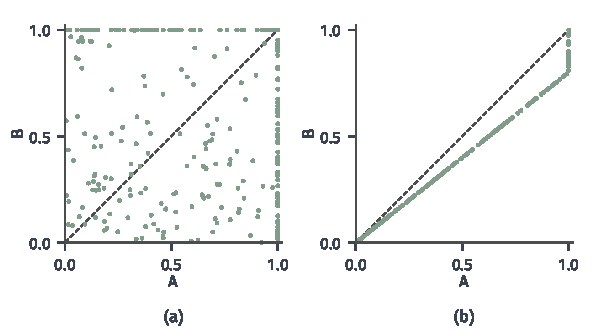
\includegraphics[width=100mm]{figures/07-probability/08-sampling-and-integration/matplotlib/vr-crn/figure.pdf}
 \caption{两个封顶等待时间$A=\min\{X_A,1\}$（$X_A\sim\operatorname{Exp}(1)$）与$B=\min\{X_B,1\}$（$X_B\sim\operatorname{Exp}(1.25)$）的$300$对样本（种子9），虚线为$A=B$。(a)两方案用独立的均匀数；(b)两方案用同一个均匀数，点落在一条递增曲线上，$A-B$的波动很小。}
 \label{fig:vr-crn}
\end{BookInlineFigure}

\paragraph{输入要按用途对齐}
复杂的模拟中，一次运行要消耗许多随机数。要让共同随机数起作用，两个方案应当在同样的用途上使用同一个随机数，例如第$k$个到达时刻都用第$k$个均匀数生成；若某个方案多消耗了一个随机数，后面的所有用途都会错位，协方差随之变小，甚至变号。

\paragraph{有限差分}
共同随机数的一个重要用途是用差商估计导数$\frac{\mathrm{d}}{\mathrm{d}\theta}\mathbb{E}[F(\theta,\bm{U})]$。两个参数值各用独立输入时，差商$\bigl(F(\theta+\delta,\bm{U})-F(\theta,\bm{U}')\bigr)/\delta$的方差约为$2\operatorname{Var}(F)/\delta^2$，$\delta$越小越糟；用同一个$\bm{U}$且$F$对$\theta$光滑时，分子约为$\delta\,\partial_\theta F(\theta,\bm{U})$，差商的方差保持有界。\BookChapterRef{chap:zeroth-order-optimization}{卷五第14章“零阶随机优化”}把这种做法称为共享样本，并分析了它在优化迭代中的作用；含参期望的导数怎样直接用样本表示，由第~\ref{chap:expectation-gradient-estimation}章研究。


\section{本章小结}
\label{sec:vr-summary}

本章固定积分$I=\mathbb{E}_P[f(X)]$，研究怎样在可比的预算下减小随机计算的波动。比较的口径是第~\ref{sec:vr-comparison}节的单元方差乘以单元成本：一种改动只有在$v\,c$变小、而且计入预备成本后仍然划算时才算改进；有偏的估计比较均方误差，并单独检查偏差是否随样本量消失。

三类方法作用在计算流水线的不同位置。改变分布调整重要贡献被抽到的频率：重要性采样按建议分布抽样、乘权重折回，理想建议正比于贡献$\lvert f\rvert p$；它在覆盖条件下无偏，但方差有限要另查加权二阶矩，尾部过轻的建议会使方差为无穷；未知归一化常数时的自归一化估计只是一致的，有限样本有偏，权重的有效样本量看不到漏掉的区域。

改变计算公式消去可以预测或可以精确平均的波动：控制变量减去回归可解释的部分，条件期望把组内波动整个算掉。改变抽样机制控制点的去向与点之间的协方差：分层去掉层间波动，拉丁超立方去掉各坐标的主效应，随机化准蒙特卡洛按Fourier频率过滤误差，对偶变量利用负协方差，共同随机数利用正协方差。

\begin{BookInlineTable}
 \centering
 \caption{本章方法在贯穿例子上的效果。单样本方差均折合到一次函数求值；“倍数”是独立抽样方差与之的比值，未计入额外成本。}
 \label{tab:vr-summary}
 \begin{tabular}{llll}
  \toprule
  方法 & 起作用的条件 & 例子 & 倍数\\
  \midrule
  重要性采样 & $q$接近$\lvert f\rvert p$ & 尾概率，$\lambda=1/4$ & $10.3$\\
  试运行拟合 & 覆盖各区，留防御成分 & 两区域尾部 & $37.7$\\
  控制变量 & $\rho^2$接近$1$ & $\mathrm{e}^{U}$，$h=U$ & $61$\\
  条件期望 & 条件平均可算 & 四分之一圆 & $3.4$\\
  比例分层 & 层均值差别大 & $\mathrm{e}^{U}$，$4$层 & $14.6$\\
  随机移位 & $F$在环面上光滑 & $\mathrm{e}^{U}$，$4$点 & $3.9$\\
  对偶变量 & 奇部方差较大 & $\mathrm{e}^{U}$ & $31$\\
  共同随机数 & 两输出正相关 & 封顶等待时间 & $67.6$\\
  \bottomrule
 \end{tabular}
\end{BookInlineTable}

表~\ref{tab:vr-summary}中的倍数只在各自的例子上成立，并且每一行都有反例：$\lambda\geq2$的指数建议、没有防御成分的拟合、交互型函数上的拉丁超立方、对称函数上的对偶对、用反向输入的共同随机数，都会使方差不降反升甚至为无穷。生成映射$T$也会改变结论，同一个光滑的$f$经过不同的$T$，随机化准蒙特卡洛的误差速度可以从$n^{-2}$降到$n^{-2/3}$。

样本不再独立时，误差估计要相应改变：整组随机化的方法以完整的一组为独立单位，用组间方差除以重复次数估计误差，不能用组内点的样本方差代替。三类操作可以组合，例如在拉丁超立方的点上再用控制变量，或在分层的每层内用重要性采样；但期望正确、方差有限与节省总计算量是三个不同的要求，组合后要重新逐项检查，各方法单独使用时的改进不能直接相乘。实际预算下怎样分配试运行与正式计算、怎样在方法之间取舍，由第~\ref{chap:sampling-budget-method-selection}章统一讨论；下一章把同样的思路用于含参期望的梯度。

